%%%%%%%%%%%%%%%%%%%%%%%%%%%%%%%%%%%%%%%%%
% Beamer Presentation
% LaTeX Template
% Version 2.0 (March 8, 2022)
%
% This template originates from:
% https://www.LaTeXTemplates.com
%
% Author:
% Vel (vel@latextemplates.com)
%
% License:
% CC BY-NC-SA 4.0 (https://creativecommons.org/licenses/by-nc-sa/4.0/)
%
%%%%%%%%%%%%%%%%%%%%%%%%%%%%%%%%%%%%%%%%%

%----------------------------------------------------------------------------------------
%	PACKAGES AND OTHER DOCUMENT CONFIGURATIONS
%----------------------------------------------------------------------------------------
\PassOptionsToPackage{dvipsnames}{xcolor}
\documentclass[
	11pt, % Set the default font size, options include: 8pt, 9pt, 10pt, 11pt, 12pt, 14pt, 17pt, 20pt
	%t, % Uncomment to vertically align all slide content to the top of the slide, rather than the default centered
	%aspectratio=169, % Uncomment to set the aspect ratio to a 16:9 ratio which matches the aspect ratio of 1080p and 4K screens and projectors
]{beamer}

\usepackage{booktabs} % Allows the use of \toprule, \midrule and \bottomrule for better rules in tables

%----------------------------------------------------------------------------------------
%	SELECT LAYOUT THEME
%----------------------------------------------------------------------------------------

% Beamer comes with a number of default layout themes which change the colors and layouts of slides. Below is a list of all themes available, uncomment each in turn to see what they look like.

%\usetheme{default}
%\usetheme{AnnArbor}
%\usetheme{Antibes}
%\usetheme{Bergen}
%\usetheme{Berkeley}
%\usetheme{Berlin}
\usetheme{Boadilla}
%\usetheme{CambridgeUS}
%\usetheme{Copenhagen}
%\usetheme{Darmstadt}
%\usetheme{Dresden}
%\usetheme{Frankfurt}
%\usetheme{Goettingen}
%\usetheme{Hannover}
%\usetheme{Ilmenau}
%\usetheme{JuanLesPins}
%\usetheme{Luebeck}
%\usetheme{Madrid}
%\usetheme{Malmoe}
%\usetheme{Marburg}
%\usetheme{Montpellier}
%\usetheme{PaloAlto}
%\usetheme{Pittsburgh}
%\usetheme{Rochester}
%\usetheme{Singapore}
%\usetheme{Szeged}
%\usetheme{Warsaw}

%----------------------------------------------------------------------------------------
%	SELECT COLOR THEME
%----------------------------------------------------------------------------------------

% Beamer comes with a number of color themes that can be applied to any layout theme to change its colors. Uncomment each of these in turn to see how they change the colors of your selected layout theme.

%\usecolortheme{albatross}
%\usecolortheme{beaver}
%\usecolortheme{beetle}
%\usecolortheme{crane}
%\usecolortheme{dolphin}
%\usecolortheme{dove}
%\usecolortheme{fly}
%\usecolortheme{lily}
%\usecolortheme{monarca}
%\usecolortheme{seagull}
%\usecolortheme{seahorse}
\usecolortheme{spruce}
%\usecolortheme{whale}
%\usecolortheme{wolverine}

%----------------------------------------------------------------------------------------
%	SELECT FONT THEME & FONTS
%----------------------------------------------------------------------------------------

% Beamer comes with several font themes to easily change the fonts used in various parts of the presentation. Review the comments beside each one to decide if you would like to use it. Note that additional options can be specified for several of these font themes, consult the beamer documentation for more information.

\usefonttheme{default} % Typeset using the default sans serif font
%\usefonttheme{serif} % Typeset using the default serif font (make sure a sans font isn't being set as the default font if you use this option!)
%\usefonttheme{structurebold} % Typeset important structure text (titles, headlines, footlines, sidebar, etc) in bold
%\usefonttheme{structureitalicserif} % Typeset important structure text (titles, headlines, footlines, sidebar, etc) in italic serif
%\usefonttheme{structuresmallcapsserif} % Typeset important structure text (titles, headlines, footlines, sidebar, etc) in small caps serif

%------------------------------------------------

%\usepackage{mathptmx} % Use the Times font for serif text
\usepackage{palatino} % Use the Palatino font for serif text
\usepackage{tikz}
\usepackage{algorithm}
\usepackage{array}
\usepackage[commentColor=grey,indLines=false,rightComments=false,noEnd=true]{algpseudocodex}
\usetikzlibrary{positioning, shapes.arrows, calc, fit, backgrounds}
\usepackage{helvet} % Use the Helvetica font for sans serif text
%\usepackage[default]{opensans} % Use the Open Sans font for sans serif text
%\usepackage[default]{FiraSans} % Use the Fira Sans font for sans serif text
%\usepackage[default]{lato} % Use the Lato font for sans serif text

\newcommand\pro{\item[$+$]}
\newcommand\con{\item[$-$]}
\definecolor{arrowcolor}{RGB}{197,224,180}
\definecolor{boxcolor}{RGB}{143,170,220}
\definecolor{lightgreen}{RGB}{74, 255, 137}
\definecolor{mixed}{RGB}{165, 225, 69}

%----------------------------------------------------------------------------------------
%	SELECT INNER THEME
%----------------------------------------------------------------------------------------

% Inner themes change the styling of internal slide elements, for example: bullet points, blocks, bibliography entries, title pages, theorems, etc. Uncomment each theme in turn to see what changes it makes to your presentation.

%\useinnertheme{default}
\useinnertheme{circles}
%\useinnertheme{rectangles}
%\useinnertheme{rounded}
%\useinnertheme{inmargin}

%----------------------------------------------------------------------------------------
%	SELECT OUTER THEME
%----------------------------------------------------------------------------------------

% Outer themes change the overall layout of slides, such as: header and footer lines, sidebars and slide titles. Uncomment each theme in turn to see what changes it makes to your presentation.

%\useoutertheme{default}
%\useoutertheme{infolines}
%\useoutertheme{miniframes}
%\useoutertheme{smoothbars}
%\useoutertheme{sidebar}
%\useoutertheme{split}
%\useoutertheme{shadow}
%\useoutertheme{tree}
%\useoutertheme{smoothtree}

%\setbeamertemplate{footline} % Uncomment this line to remove the footer line in all slides
%\setbeamertemplate{footline}[page number] % Uncomment this line to replace the footer line in all slides with a simple slide count

%\setbeamertemplate{navigation symbols}{} % Uncomment this line to remove the navigation symbols from the bottom of all slides

%----------------------------------------------------------------------------------------
%	PRESENTATION INFORMATION
%----------------------------------------------------------------------------------------

\title[CaVieR]{CaVieR} % The short title in the optional parameter appears at the bottom of every slide, the full title in the main parameter is only on the title page

\subtitle{CAscading VIew tRees} % Presentation subtitle, remove this command if a subtitle isn't required

\author[Johann Schwabe]{Johann Schwabe} % Presenter name(s), the optional parameter can contain a shortened version to appear on the bottom of every slide, while the main parameter will appear on the title slide

\institute[UZH]{University of Zurich\\ \smallskip \textit{johann.schwabe@uzh.ch}} % Your institution, the optional parameter can be used for the institution shorthand and will appear on the bottom of every slide after author names, while the required parameter is used on the title slide and can include your email address or additional information on separate lines

\date[\today]{Master Thesis Defence \\ \today} % Presentation date or conference/meeting name, the optional parameter can contain a shortened version to appear on the bottom of every slide, while the required parameter value is output to the title slide

%----------------------------------------------------------------------------------------

\begin{document}

%----------------------------------------------------------------------------------------
%	TITLE SLIDE
%----------------------------------------------------------------------------------------

\begin{frame}
	\titlepage % Output the title slide, automatically created using the text entered in the PRESENTATION INFORMATION block above
\end{frame}

%----------------------------------------------------------------------------------------
%	TABLE OF CONTENTS SLIDE
%----------------------------------------------------------------------------------------

% The table of contents outputs the sections and subsections that appear in your presentation, specified with the standard \section and \subsection commands. You may either display all sections and subsections on one slide with \tableofcontents, or display each section at a time on subsequent slides with \tableofcontents[pausesections]. The latter is useful if you want to step through each section and mention what you will discuss.

%----------------------------------------------------------------------------------------
%	PRESENTATION BODY SLIDES
%----------------------------------------------------------------------------------------



\section{Introduction}
\begin{frame}
	\frametitle{Introduction}
	\framesubtitle{Real time data analytics}
	\begin{enumerate}
		\item Different aspects of the data
		\item Real time
		\item Big Data
	\end{enumerate}
	\footnotetext{\tiny{Image by @kamrulhkhkhk https://de.freepik.com}}
\end{frame}

\begin{frame}
	\frametitle{Introduction}
	\framesubtitle{Naive Approach}
	Consider the query $Q$ which joins the four relations R, S, T and U:
	$Q = R, S, T, U$\\
	\vspace{1cm}
	Naive approach: Recompute on change
	\begin{enumerate}
		\pro simple
		\con very slow
	\end{enumerate}
\end{frame}
\begin{frame}
	\frametitle{Introduction}
	\framesubtitle{Classical IVM}
	Consider the query $Q$ which joins the four relations R, S, T and U:
	$Q = R, S, T, U$\\
	\vspace{1cm}
	Classical IVM
	\begin{enumerate}
		\pro only computes the change
		\con still slow
	\end{enumerate}
	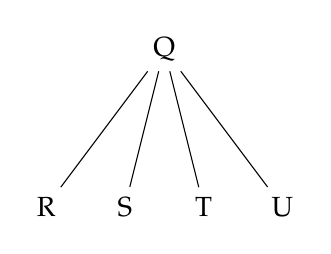
\begin{tikzpicture}
		[level distance=2cm,
		sibling distance=1cm]
		\node {Q}
		child {node {R}}
		child {node {S}}
		child {node {T}}
		child {node {U}};
	\end{tikzpicture}
	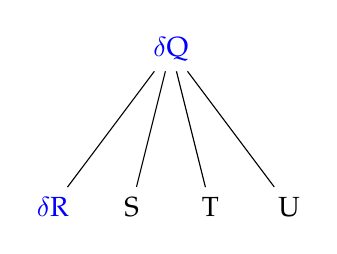
\begin{tikzpicture}
			[level distance=2cm,
		sibling distance=1cm]
		\node {\textcolor{blue}{$\delta$Q}}
		child {node {\textcolor{blue}{$\delta$R}}}
		child {node {S}}
		child {node {T}}
		child {node {U}};
	\end{tikzpicture}
%	\begin{tikzpicture}[remember picture,overlay]
%		\node[anchor=south west, yshift=0cm] at (current page.south west) {\includegraphics[width=\paperwidth,trim={0 0 0 1.5cm},clip]{Figures/IntroClassical.pdf}};
%	\end{tikzpicture}
\end{frame}

\begin{frame}
	\frametitle{Introduction}
	\framesubtitle{DBToaster}
	Consider the query $Q$ which joins the four relations R, S, T and U:
	$Q = R, S, T, U$\\
	\vspace{1cm}
	DBToaster
	\begin{enumerate}
		\pro reuses partial joins
		\con many views to maintain
	\end{enumerate}
	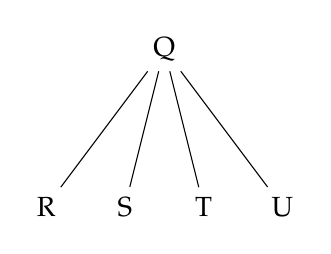
\begin{tikzpicture}
		[level distance=2cm,
		sibling distance=1cm]
		\node {Q}
		child {node {R}}
		child {node {S}}
		child {node {T}}
		child {node {U}};
	\end{tikzpicture}
	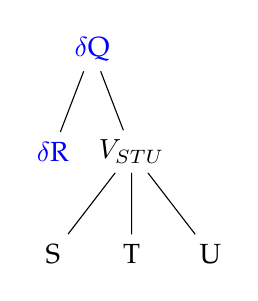
\begin{tikzpicture}
		[level distance=1.3cm,
		sibling distance=1cm]
		\node {\textcolor{blue}{$\delta$Q}}
		child {node {\textcolor{blue}{$\delta$R}}}
		child {node {$\text{V}_{\text{STU}}$}
		child {node {S}}
		child {node {T}}
		child {node {U}}
		};
	\end{tikzpicture}
	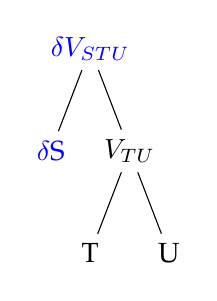
\begin{tikzpicture}
		[level distance=1.3cm,
		sibling distance=1cm]
		\node {\textcolor{blue}{$\delta\text{V}_{\text{STU}}$}}
		child {node {\textcolor{blue}{$\delta$S}}}
		child {node {$\text{V}_{\text{TU}}$}
			child {node {T}}
			child {node {U}}
		};
	\end{tikzpicture}
\end{frame}

\begin{frame}
	\frametitle{Introduction}
	\framesubtitle{F-IVM}
	Consider the query $Q$ which joins the four relations R, S, T and U:
	$Q = R, S, T, U$\\
	\vspace{1cm}
	F-IVM
	\begin{enumerate}
		\pro fewer views to be maintained
		\pro can be asymptotically faster
		\con supports only a single query
	\end{enumerate}
	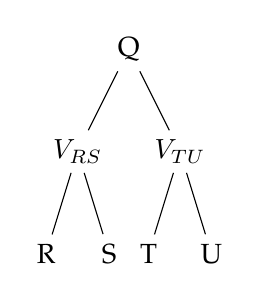
\begin{tikzpicture}
		[level distance=1.3cm,
		sibling distance=1.3cm,
		level 2/.style={sibling distance=0.8cm}]
		\node {Q}
		child {node {$\text{V}_{\text{RS}}$}
			child {node {R}}
			child {node {S}}
		}
		child {node {$\text{V}_{\text{TU}}$}
			child {node {T}}
			child {node {U}}
		};
	\end{tikzpicture}
	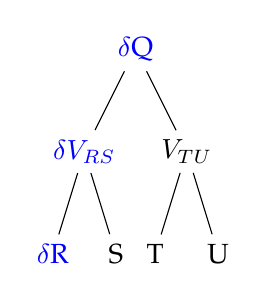
\begin{tikzpicture}
		[level distance=1.3cm,
		sibling distance=1.3cm,
		level 2/.style={sibling distance=0.8cm}]
		\node {\textcolor{blue}{$\delta$Q}}
		child {node {\textcolor{blue}{$\delta\text{V}_{\text{RS}}$}}
			child {node {\textcolor{blue}{$\delta$R}}}
			child {node {S}}
		}
		child {node {$\text{V}_{\text{TU}}$}
			child {node {T}}
			child {node {U}}
		};
	\end{tikzpicture}
\end{frame}

\begin{frame}
	\frametitle{Introduction}
	\framesubtitle{Redundant computation}
	Processing queries with idendical subtrees individually results in redundant computation\\
	\vspace{1cm}
		\begin{minipage}{0.49\textwidth}
		\centering
	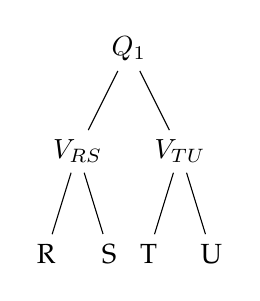
\begin{tikzpicture}
		[level distance=1.3cm,
		sibling distance=1.3cm,
		level 2/.style={sibling distance=0.8cm}]
		\node {$\text{Q}_\text{1}$}
		child {node {$\text{V}_{\text{RS}}$}
			child {node {R}}
			child {node {S}}
		}
		child {node {$\text{V}_{\text{TU}}$}
			child {node {T}}
			child {node {U}}
		};
	\end{tikzpicture}
		\end{minipage}
	\begin{minipage}{0.49\textwidth}
	\centering
	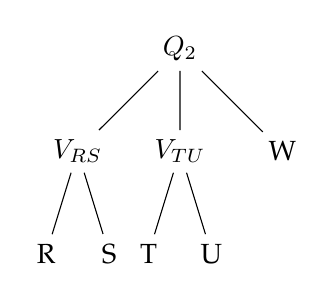
\begin{tikzpicture}
		[level distance=1.3cm,
		sibling distance=1.3cm,
		level 2/.style={sibling distance=0.8cm}]
		\node {$\text{Q}_\text{2}$}
		child {node {$\text{V}_{\text{RS}}$}
			child {node {R}}
			child {node {S}}
		}
		child {node {$\text{V}_{\text{TU}}$}
			child {node {T}}
			child {node {U}}
		}
		child {node {W}};
	\end{tikzpicture}
		\end{minipage}
\end{frame}

\begin{frame}
	\frametitle{Introduction}
	\framesubtitle{Improving performance by shared query maintenance}
	Reusing identical subtrees reduces redundant computation
	
	This can reduce the asymptotic complexity. In some cases, non q-hierarchical queries can be executed at the speed of q-hierarchical queries.\\
	\vspace{1cm}
	\begin{minipage}{0.49\textwidth}
		\centering
			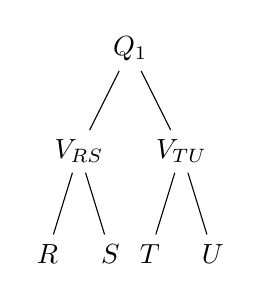
\begin{tikzpicture}[
			level distance=1.3cm,
			level 1/.style={sibling distance=1.3cm},
			level 2/.style={sibling distance=0.8cm}
			]
			
			% Nodes
			\node (Q1) {$\text{Q}_\text{1}$}
			child {node (VRS) {$\text{V}_\text{RS}$}
				child {node (R) {$\text{R}$}}
				child {node (S) {$\text{S}$}}
			}
			child {node (VTU) {$\text{V}_\text{TU}$}
				child {node (T) {$\text{T}$}}
				child {node (U) {$\text{U}$}}
			};
		\end{tikzpicture}
	\end{minipage}
	\begin{minipage}{0.49\textwidth}
				\centering
		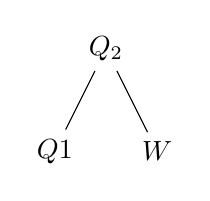
\begin{tikzpicture}[
			level distance=1.3cm,
			level 1/.style={sibling distance=1.3cm},
			level 2/.style={sibling distance=0.8cm}
			]
			
			% Nodes
			\node (Q2) {$\text{Q}_\text{2}$}
			child {node (Q1) {$\text{Q1}$}}
			child {node (W) {$\text{W}$}};
			
		\end{tikzpicture}
	\end{minipage}
\end{frame}


\begin{frame}
	\frametitle{Example}
	\framesubtitle{Query Rewriting}
		\begin{align*}
			Q_2(y,z) =&\ R_1(x, y), \colorbox{yellow}{\mbox{$R_2(y,z,w,v), R_3(y,w)$}}\\
			Q_1(y,w,z) =&\  \colorbox{yellow}{\mbox{$R_2(y,z,w,v), R_3(y,w)$}}\\
%			Q_1'(y,z) =&\ Q_2(y,w,z), R_1(x, y)
		\end{align*}

\end{frame}

%\begin{frame}
%	\frametitle{Foundation}
%	\framesubtitle{Query Rewriting}
%			Following [Geck et al., 2022]\footnote{Geck, G., Keppeler, J., Schwentick, T., and Spinrath, C. (2022). Rewriting with acyclic queries: Mind your head. CoRR, abs/2201.05129.}:
%	\begin{align*}
%		Q_2(y,z) =&\ \colorbox{cyan}{\mbox{$R_1(x, y)$}}, \colorbox{yellow}{\mbox{$R_2(y,z,w,v), R_3(y,w)$}}\\
%		Q_1(y,w,z) =&\ \colorbox{yellow}{\mbox{$R_2(y,z,w,v), R_3(y,w)$}}\\
%		%			Q_1'(y,z) =&\ Q_2(y,w,z), R_1(x, y)
%	\end{align*}
%	
%\end{frame}



\begin{frame}
	\frametitle{Example}
	\framesubtitle{Query Rewriting}
	\begin{align*}
		Q_2(y,z) =&\ R_1(x, y), R_2(y,z,w,v), R_3(y,w)\\
		Q_1(y,w,z) =&\ R_2(y,z,w,v), R_3(y,w)\\\\
		Q_2'(y,z) =&\ R_1(x, y), Q_1(y,w,z)
	\end{align*}
\end{frame}

\begin{frame}
	\frametitle{Example}
	\framesubtitle{From dependency graph to a cascading view tree}
	\vspace{-0.4cm}
	\begin{align*}
		Q_1(y,w,z) =&\ R_2(y,z,w,v), R_3(y,w)\\
		Q_2'(y,z) =&\ R_1(x, y), Q_1(y,w,z)
	\end{align*}
	\begin{minipage}{0.45\textwidth}
		\centering
			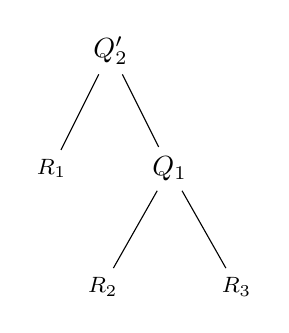
\begin{tikzpicture}[
			level distance=1.5cm,
			level 2/.style={sibling distance=1.7cm}]
			\node {$Q_2'$}
			child {node {\footnotesize \texttt{$R_1$}}}
			child {node {$Q_1$}
				child {node {\footnotesize \texttt{$R_2$}}}
				child {node {\footnotesize \texttt{$R_3$}}}
			};
		\end{tikzpicture}
	\end{minipage}
	\begin{minipage}{0.45\textwidth}
		\centering
		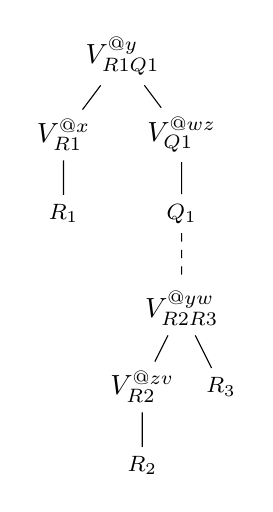
\begin{tikzpicture}[
			level distance=1cm,
			level 2/.style={sibling distance=1cm},
			level 3/.style={level distance=1.2cm},
			level 4/.style={level distance=1cm}
			]
			\node {$V_{R1Q1}^{@y}$}
			child {node {$V_{R1}^{@x}$}
				child {node {\footnotesize \texttt{$R_1$}}}
			}
			child {node {$V_{Q1}^{@wz}$}
				child {node {\footnotesize \texttt{$Q_1$}}
					child[dashed] {node {$V_{R2R3}^{@yw}$}
						child[solid] {node {$V_{R2}^{@zv}$}
							child{node{\footnotesize \texttt{$R_2$}}}
						}
						child[solid]{node{\footnotesize \texttt{$R_3$}}}
					}
				}
			};
		\end{tikzpicture}
	\end{minipage}
	

\end{frame}

%\begin{frame}
%	\frametitle{Motivating Example II}
%	\framesubtitle{CaVieR}
%	\begin{columns}
%		\begin{column}{0.3\textwidth}
%			\begin{align*}
%				Q_1 &= R_1, R_2, R_3, R_4, R_5\\
%				Q_2 &= R_1, R_2, R_3\\
%				Q_3 &= R_2, R_3\\
%				Q_4 &= R_3, R_4, R_5\\
%				Q_5 &= R_3, R_4
%			\end{align*}
%		\end{column}
%		
%		\begin{column}{0.7\textwidth}
%			\begin{figure}
%				\includegraphics[width=0.76\linewidth, trim=0 1.5cm 0 1.5cm, clip]{Figures/Viz_DoubleR3.pdf}
%			\end{figure}
%		\end{column}
%		
%	\end{columns}
%\end{frame}


%------------------------------------------------


%
%\subsection{Foundations}
%\begin{frame}
%		\frametitle{Foundations}
%		\framesubtitle{Principles of FIVM}
%
%
%		$Q_1(y,z) = R_1(x, y), R_2(y,z,w,v), R_3(y,w)$
%		\begin{columns}[c] 
%			\begin{column}{0.45\textwidth} 
%				\begin{figure}
%					\includegraphics[height=0.5\textheight]{Figures/variable_order.pdf}
%					\caption{Variable Order}
%				\end{figure}
%			\end{column}
%			\begin{column}{0.45\textwidth} 
%				\begin{figure}
%					\includegraphics[height=0.5\textheight]{Figures/optimized_viewtree.pdf}
%					\caption{View Tree}
%				\end{figure}
%			\end{column}
%		\end{columns}
%\end{frame}
%
%\begin{frame}
%	\frametitle{Dynamic Query Evaluation Framework}
%	\framesubtitle{[Kara et al., 2023]}
%	\scriptsize
%	\vspace*{-0.5cm}
%	Given a CQAP $Q(\mathcal{O} \mid \mathcal{I})$, compute a data structure that supports answering the access requests and maintains it under updates. 
%
%	\begin{figure}
%		\hspace*{-2cm}
%		\centering
%		\begin{tikzpicture}
%			\node at (-1.0,-0.25) {query};
%			\node at (1.0,-0.05) {data};
%			\node at (1.0,-0.4) {base};
%			\node at (5.5,-0.3){
%				\begin{tikzpicture}
%					\tikzstyle{background}=[rectangle, rounded corners=2mm]
%					\fill[rounded corners=2mm, fill=blue!20,inner sep= 2.5mm] (0,0) rectangle (2,1.5) node[pos=.5, text width=2cm, align=center] {data structure};
%				\end{tikzpicture}
%			};
%			
%			\node at (1.8, -0.3) (anchor1''){};
%			\node at (4.2, -0.3) (anchor2''){};
%			\node at (3, 0.1) {preprocess};
%			
%			\draw[->,color = blue,minimum height=4cm,minimum width=7cm, line width = 0.07cm](anchor1'')-- (anchor2'');
%			
%			\node at (3, -0.7) {\em \color{OliveGreen} preprocessing};
%			\node at (3, -1.1) {\em \color{OliveGreen} time};
%			
%			%%%%%%%%%%%%%%%
%			% Enumeration
%			%%%%%%%%%%%%%%% 
%				\node at (7.8, -1.0) {enumerate};
%				\draw[dashed,->,color = blue,minimum height=4cm,minimum width=7cm, line width = 0.07cm](6.8,-0.6)-- (8.8,-0.6);
%				\node at (10.5,-1.9cm){
%					\begin{tikzpicture}
%						\tikzstyle{background}=[rectangle, rounded corners=2mm]
%						\fill[rounded corners=2mm, fill=blue!20,inner sep= 2.5mm] (0,0) rectangle (1.75,2.2) node[pos=.5, text width=3cm, align=center] {};
%							\node at (0.85, 1.9) {tuple 1};
%						
%							\node at (0.85, 1.45) {tuple 2};
%
%							\node at (0.85, 1.05) {$\dots$};
%
%							\node at (0.85, 0.7) {tuple n};
%
%							\node[text width=2cm, align=center] at (2.75, 0.7) {\em \color{OliveGreen} enumeration delay};
%
%							\node at (0.85, 0.3) {EOF};
%
%						
%						\node at (0.85, -0.5) {$\mathcal{O}$-tuples};
%						% \node at (0.85, -0.8) {EOF};
%					\end{tikzpicture}
%				};
%				
%				% 
%				\node[text width=2cm, align=center] at (7.8, 0.8) {access request};
%				\draw[<-,color = blue,minimum height=4cm,minimum width=7cm, line width = 0.07cm](6.8,0.3)-- (8.8,0.3);
%				\node at (9.8,0.3cm){
%					$\mathcal{I}$-tuple
%				};
%
%			%%%%%%%%%%%%%%%
%			% Single-tuple update
%			%%%%%%%%%%%%%%
%				\node at (0.97, -3.3) (anchor1''''){};
%				\node at (0.97, -0.7) (anchor2''''){};
%				\node at (0.97, -3.7) {update};
%				% \node at (0.57, -3.9) {tuples};
%				
%				\draw[->,color = blue,minimum height=4cm,minimum width=7cm, line width = 0.07cm](anchor1'''')-- (anchor2'''');
%				\node at (1.9, -3.7) (anchor3){};
%				\node at (5.5, -3.7) (anchor4){};
%				\node at (5.4, -3.85) (anchor42){};
%				\node at (5.4, -1.1) (anchor5){};
%				
%				\draw[color = blue,minimum height=4cm,minimum width=7cm, line width = 0.07cm](anchor3)-- (anchor4);
%				
%				\draw[->,color = blue,minimum height=4cm,minimum width=7cm, line width = 0.07cm](anchor42)-- (anchor5);
%				
%				\node at (3.5, -3.4) {maintain};
%				
%				
%				\node[rotate=90] at (0.65, -2.0) {\footnotesize maintain};
%				
%				
%				\node at (3.5, -4.0) {\em \color{OliveGreen} update time};
%				
%				\node[rotate=90] at (1.3, -2.0) {\footnotesize \em \color{OliveGreen} update time};
%		\end{tikzpicture}
%		
%		
%	\end{figure}
%	
%\end{frame}
%
%\begin{frame}
%	\frametitle{Foundations}
%	\framesubtitle{Query Classes}
%	Complexity of Conjunctive Queries:
%	\begin{align*}
%		Preprocessing Time & & O(N^w) \\
%		Enumeration Delay & & O(1) \\
%		Update Time & & O(N^\delta)
%	\end{align*}
%	$w$: Fractional Hypertree Width\\
%	$\delta$: largest $w$ over all delta queries
%	\begin{block}{Q-Hierarchical}
%		$w = 1, \delta=0$ 
%	\end{block}
%\end{frame}
\begin{frame}
	\frametitle{CaVieR}
	\framesubtitle{Definition}
	Given a set of Cascading Q-Hierarchical Queries, CaVieR:
	\begin{enumerate}
		\item  computes a Cascading Q-Hierarchical Rewriting
		\item  generates a cascading view tree
		\item  supports dynamic evaluation with
		\begin{itemize}
			\item constant update time
			\item constant enumeration delay
		\end{itemize}
	\end{enumerate}
	
	Therefor, CaVieR can be asymptotically faster than individual F-IVM instances
\end{frame}


\section{CaVieR}
\subsection{Aim}
\begin{frame}
	\frametitle{CaVieR}
	\framesubtitle{Aim of the Thesis}
	\begin{enumerate}
		\item Developping CaVieR
		\item Implementing CaVieR
		\item Testing CaVieR on synthetic and real-world datasets
	\end{enumerate}
\end{frame}

\subsection{Algorithm}
\begin{frame}
	\frametitle{CaVieR }
	\framesubtitle{Algorithm}
	\centering
	\includegraphics[height=0.8\textheight]{Figures/Algo.png}
\end{frame}

\begin{frame}
	\frametitle{CaVieR}
	\framesubtitle{Homomorphism}
	\begin{block}{Homomorphism [Chandra and Merlin, 1977]}
		$Q_1 \sqsupseteq Q_2$ implies that there is a mapping $h: \texttt{vars}(Q_2) \rightarrow \texttt{vars}(Q_1)$ such that $h(\texttt{body}(Q_2)) \subseteq \texttt{body}(Q_1)$ and $h(\texttt{head}(Q_2)) \subseteq \texttt{head}(Q_1)$. 
	\end{block}
\end{frame}

\begin{frame}
	\frametitle{CaVieR}
	\framesubtitle{Single Query Rewriting}
	\textbf{Input}: Query q, Set[Query] V
	\begin{enumerate}
		\item Iterate over each partition the body of q
		\item Iterate over each element of the partition
		\item Find homomorphism for the element to a query in V
		\item If homomorphism is found for every element, check if the resulting query is q-hierarchical
	\end{enumerate}
	\textbf{Output}: Set[Queries] - all rewritings of q
\end{frame}


%\begin{frame}
%	\frametitle{CaVieR}
%	\framesubtitle{Single Query Rewriting}
%	\begin{algorithm}[H]
%		\caption{Single Rewriting (\textit{Simplified})}\label{alg:SingleRewriting}
%		\begin{algorithmic}[1]
%			\Function{SingleRewriting}{views: Set[Query], q: Query}
%			\For{$(A_1,...,A_m) \in Partitions(body(q))$}
%			\For{$A_i \in A_1,...,A_m$}
%			\State $morph_i \gets$ FindHomomorphism($A_i$, views)\footnotemark
%			\If{$morph_i$ == Null}
%			\State \textbf{break}
%			\EndIf
%			\EndFor
%			\If{isQHierarchical(\{$morph_1,\dots,morph_m$\})}
%			\State \textbf{report} \{$morph_1,\dots,morph_m$\}
%			\EndIf
%			\EndFor
%			\EndFunction
%		\end{algorithmic}
%	\end{algorithm}
%	\footnotetext{Cover Partition by Geck, G., Keppeler, J., Schwentick, T., and Spinrath, C. (2022). Rewriting with acyclic queries: Mind your head. CoRR, abs/2201.05129.}
%\end{frame}
\begin{frame}
	\frametitle{CaVieR}
	\framesubtitle{Single Query Rewriting Example}
	\begin{align*}
		Q_2(x,y,z,w) &= R_1(x,y), R_2(y,z), R_3(z,w) &\\
		Q_3(y,z,w) &= R_2(y,z), R_3(z,w)&\\
	\end{align*}
	\textbf{Input}: $Q_2$, $\{Q_3\}$
	\vspace{4cm}
\end{frame}

\begin{frame}
	\frametitle{CaVieR}
	\framesubtitle{Single Query Rewriting Example}
	\begin{align*}
		Q_2(x,y,z,w) &= R_1(x,y), R_2(y,z), R_3(z,w) &\\
		Q_3(y,z,w) &= R_2(y,z), R_3(z,w)&\\
	\end{align*}
	\textbf{Input}: $Q_2$, $\{Q_3\}$
	\begin{enumerate}
		\item Iterate over each partition the body of q
	\end{enumerate}
	$Partitioning_1 = \{\{R_1\}, \{R_2, R_3\}\}$
	\vspace{3cm}
\end{frame}
\begin{frame}
	\frametitle{CaVieR}
	\framesubtitle{Single Query Rewriting Example}
	\begin{align*}
		Q_2(x,y,z,w) &= R_1(x,y), R_2(y,z), R_3(z,w) &\\
		Q_3(y,z,w) &= R_2(y,z), R_3(z,w)&\\
	\end{align*}
	\textbf{Input}: $Q_2$, $\{Q_3\}$\\
	\textbf{Variables}:
	$Partitioning_1 = \{\{R_1\}, \{R_2, R_3\}\}$
	\begin{enumerate}
		\setcounter{enumi}{1}
		\item Iterate over each element of the partition
	\end{enumerate}
	$element_1 = \{R_1\}$
	\vspace{3cm}
\end{frame}

\begin{frame}
	\frametitle{CaVieR}
	\framesubtitle{Single Query Rewriting Example}
	\begin{align*}
		Q_2(x,y,z,w) &= R_1(x,y), R_2(y,z), R_3(z,w) &\\
		Q_3(y,z,w) &= R_2(y,z), R_3(z,w)&\\
	\end{align*}
	\textbf{Input}: $Q_2$, $\{Q_3\}$\\
	\textbf{Variables}:
	$Partitioning_1 = \{\{R_1\}, \{R_2, R_3\}\}$,
	$element_1 = \{R_1\}$
	\begin{enumerate}
		\setcounter{enumi}{2}
		\item Find homomorphism for the element to a query in V
	\end{enumerate}
	Size one elements are ignored
	\vspace{3cm}
\end{frame}

\begin{frame}
	\frametitle{CaVieR}
	\framesubtitle{Single Query Rewriting Example}
	\begin{align*}
		Q_2(x,y,z,w) &= R_1(x,y), R_2(y,z), R_3(z,w) &\\
		Q_3(y,z,w) &= R_2(y,z), R_3(z,w)&
	\end{align*}
	\textbf{Input}: $Q_2$, $\{Q_3\}$\\
	\textbf{Variables}:
	$Partitioning_1 = \{\{R_1\}, \{R_2, R_3\}\}$
	\begin{enumerate}
		\setcounter{enumi}{1}
		\item Iterate over each element of the partition
	\end{enumerate}
	$element_2 = \{R_2, R_3\}$
	\vspace{3cm}
\end{frame}

\begin{frame}
	\frametitle{CaVieR}
	\framesubtitle{Single Query Rewriting Example}
	\begin{align*}
		Q_2(x,y,z,w) &= R_1(x,y), \colorbox{lightgreen}{$R_2(y,z), R_3(z,w)$} &\\
		Q_3(y,z,w) &=\colorbox{lightgreen}{$R_2(y,z), R_3(z,w)$}&
	\end{align*}
	\textbf{Input}: $Q_2$, $\{Q_3\}$\\
	\textbf{Variables}:
	$Partitioning_1 = \{\{R_1\}, \{R_2, R_3\}\}$,
	$element_2 = \{R_2, R_3\}$
	\begin{enumerate}
		\setcounter{enumi}{2}
		\item Find homomorphism for the element to a query in V
	\end{enumerate}
	Homomorphism between $element_2\ \&\ Q_3$
	\vspace{3cm}
\end{frame}


\begin{frame}
	\frametitle{CaVieR}
	\framesubtitle{Single Query Rewriting Example}
	\begin{align*}
		Q_2(x,y,z,w) &= R_1(x,y), R_2(y,z), R_3(z,w) &\\
		Q_3(y,z,w) &= R_2(y,z), R_3(z,w)&
	\end{align*}
	\textbf{Input}: $Q_2$, $\{Q_3\}$\\
	\textbf{Variables}:
	$Partitioning_1 = \{\{R_1\}, \{R_2, R_3\}\}$
	\begin{enumerate}
		\setcounter{enumi}{3}
		\item If homomorphism is found for every element, check if the resulting query is q-hierarchical
	\end{enumerate}
	Resulting query $Q_2'(x,y,z,w) = R_1(x,y), Q_3(y,z,w)$ is q-hierarchical
	\vspace{3cm}
\end{frame}

\begin{frame}
	\frametitle{CaVieR}
	\framesubtitle{Single Query Rewriting Example}
	\begin{align*}
		Q_2(x,y,z,w) &= R_1(x,y), R_2(y,z), R_3(z,w) &\\
		Q_3(y,z,w) &= R_2(y,z), R_3(z,w)&\\
	\end{align*}
	\textbf{Input}: $Q_2$, $\{Q_3\}$
	\begin{enumerate}
		\item Iterate over each partition the body of q
	\end{enumerate}
	$Partitioning_24= \dots$
	\vspace{3cm}
\end{frame}

%
%\begin{frame}
%	\frametitle{CaVieR}
%	\framesubtitle{Single Query Rewriting}
%	\begin{figure}
%		\begin{align*}
%			Q_2(x,y,z,w) &= R_1(x,y), R_2(y,z), R_3(z,w) &\\
%			Q_3(y,z,w) &= R_2(y,z), R_3(z,w)&\\
%			Q_2'(x,y,z,w)& = R_1(x,y), Q_3(y,z,w)&
%		\end{align*}
%		\vspace{1cm}
%		Solution: $\{Q_2', Q_3\}$
%	\end{figure}
%\end{frame}

%\begin{frame}
%	\frametitle{CaVieR}
%	\framesubtitle{Query Set Rewriting}
%	\begin{algorithm}[H]
%		\caption{All Rewritings (\textit{Simplified})}\label{alg:AllRewriting}
%		\begin{algorithmic}[1]
%			\Function{AllRewritings}{queries: Set[Query]}
%			\For{$query_i \in queries$}
%			\If{not isQHierarchical(query)}
%			\State{$rewritings_i \gets SingleRewriting(queries \setminus query_i, query_i)$}
%			\If{$rewritings_i.empty()$}
%			\State{\textbf{return} set()}
%			\EndIf
%			\Else
%			\State{$rewritings_i \gets \{query_i\}$}
%			\EndIf
%			\EndFor
%			\State{\textbf{return} $rewriting_1 \times \dots \times rewriting_n$}
%			\EndFunction
%		\end{algorithmic}
%	\end{algorithm}
%\end{frame}

\begin{frame}
	\frametitle{CaVieR}
	\framesubtitle{Query Set Rewriting}
	\textbf{Input}: Set[Query] V
	\begin{enumerate}
		\item Iterate over each non q-hierarchical query q in V
		\item Call SingleQueryRewriting with q and $\text{V} \setminus \text{q}$
		\item If no rewriting is found, return empty set
		\item Return cartesian product of all rewritings
	\end{enumerate}
	\textbf{Output}: Set[Set[Queries]] - all cascading q-hierarchical rewritings for V
\end{frame}


\begin{frame}
	\frametitle{CaVieR}
	\framesubtitle{Query Set Rewriting}
	\begin{tabular}{cccccc}
		\color{red}$Q_1(x,y,z,w,v)$ &\color{red}=& \color{red}$R_1(x,y),$&\color{red}$R_2(y,z),$&\color{red} $R_3(z,w), $&\color{red}$R_4(w,v)$\\
		$Q_2(x,y,z,w)$ &=& $R_1(x,y),$&$R_2(y,z),$&$R_3(z,w)$&\\
		$Q_3(y,z,w)$ &=&& $R_2(y,z),$&$ R_3(z,w)$&\\
		$Q_4(x,y,z)$ &=& $R_1(x,y),$&$ R_2(y,z)$&&\\
	\end{tabular}\\
	\vspace{1cm}
	\textbf{Input}: $\{Q_1, Q_2, Q_3, Q_4\}$\\
	\textbf{Variables}:
	\begin{enumerate}
		\setcounter{enumi}{0}
		\item Iterate over each non q-hierarchical query q in V
	\end{enumerate}
	$q = Q_1$
\end{frame}

\begin{frame}
	\frametitle{CaVieR}
	\framesubtitle{Query Set Rewriting}
	\begin{tabular}{cccccc}
		\color{red}$Q_1(x,y,z,w,v)$ &\color{red}=& \color{red}$R_1(x,y),$&\color{red}$R_2(y,z),$&\color{red} $R_3(z,w), $&\color{red}$R_4(w,v)$\\
		$Q_2(x,y,z,w)$ &=& $R_1(x,y),$&$R_2(y,z),$&$R_3(z,w)$&\\
		$Q_3(y,z,w)$ &=&& $R_2(y,z),$&$ R_3(z,w)$&\\
		$Q_4(x,y,z)$ &=& $R_1(x,y),$&$ R_2(y,z)$&&\\
	\end{tabular}\\
	\vspace{1cm}
	\textbf{Input}: $\{Q_1, Q_2, Q_3, Q_4\}$\\
	\textbf{Variables}:	$q = Q_1$
	\begin{enumerate}
		\setcounter{enumi}{1}
		\item Call SingleQueryRewriting with q and $\text{V} \setminus \text{q}$
	\end{enumerate}
	SingleQueryRewriting($Q_1, \{Q_2, Q_3, Q_4\}$)\\
	$rewritingQ_1 = \{Q_1'\}$
	\begin{align*}
		Q_1'(x,y,z,w,v) =&\ Q_2(x,y,z,w), R_4(w,v)&\\
	\end{align*}
\end{frame}

\begin{frame}
	\frametitle{CaVieR}
	\framesubtitle{Query Set Rewriting}
	\begin{tabular}{cccccc}
		\color{red}$Q_1(x,y,z,w,v)$ &\color{red}=& \color{red}$R_1(x,y),$&\color{red}$R_2(y,z),$&\color{red} $R_3(z,w), $&\color{red}$R_4(w,v)$\\
		$Q_2(x,y,z,w)$ &=& $R_1(x,y),$&$R_2(y,z),$&$R_3(z,w)$&\\
		$Q_3(y,z,w)$ &=&& $R_2(y,z),$&$ R_3(z,w)$&\\
		$Q_4(x,y,z)$ &=& $R_1(x,y),$&$ R_2(y,z)$&&\\
	\end{tabular}\\
	\vspace{1cm}
	\textbf{Input}: $\{Q_1, Q_2, Q_3, Q_4\}$\\
	\textbf{Variables}:	$q = Q_1$, 	$rewritingQ_1 = \{Q_1'\}$
	\begin{enumerate}
		\setcounter{enumi}{2}
		\item If no rewriting is found, return empty set
	\end{enumerate}
	$rewritingQ_1 \neq \emptyset$ $\rightarrow$ continue
\end{frame}

\begin{frame}
	\frametitle{CaVieR}
	\framesubtitle{Query Set Rewriting}
	\begin{tabular}{cccccc}
		$Q_1(x,y,z,w,v)$ &=& $R_1(x,y),$&$R_2(y,z),$& $R_3(z,w), $&$R_4(w,v)$\\
		\color{red}$Q_2(x,y,z,w)$ &\color{red}=& \color{red}$R_1(x,y),$&\color{red}$R_2(y,z),$&\color{red}$R_3(z,w)$&\\
		$Q_3(y,z,w)$ &=&& $R_2(y,z),$&$ R_3(z,w)$&\\
		$Q_4(x,y,z)$ &=& $R_1(x,y),$&$ R_2(y,z)$&&\\
	\end{tabular}\\
	\vspace{1cm}
	\textbf{Input}: $\{Q_1, Q_2, Q_3, Q_4\}$\\
	\textbf{Variables}:
	\begin{enumerate}
		\setcounter{enumi}{0}
		\item Iterate over each non q-hierarchical query q in V
	\end{enumerate}
	$q = Q_2$
\end{frame}

\begin{frame}
	\frametitle{CaVieR}
	\framesubtitle{Query Set Rewriting}
	\begin{tabular}{cccccc}
		$Q_1(x,y,z,w,v)$ &=& $R_1(x,y),$&$R_2(y,z),$& $R_3(z,w), $&$R_4(w,v)$\\
		\color{red}$Q_2(x,y,z,w)$ &\color{red}=& \color{red}$R_1(x,y),$&\color{red}$R_2(y,z),$&\color{red}$R_3(z,w)$&\\
		$Q_3(y,z,w)$ &=&& $R_2(y,z),$&$ R_3(z,w)$&\\
		$Q_4(x,y,z)$ &=& $R_1(x,y),$&$ R_2(y,z)$&&\\
	\end{tabular}\\
	\vspace{1cm}
	\textbf{Input}: $\{Q_1, Q_2, Q_3, Q_4\}$\\
	\textbf{Variables}:	$q = Q_2$
	\begin{enumerate}
		\setcounter{enumi}{1}
		\item Call SingleQueryRewriting with q and $\text{V} \setminus \text{q}$
	\end{enumerate}
	SingleQueryRewriting($Q_2, \{Q_1, Q_3, Q_4\}$)\\
	$rewritingQ_2 = \{Q_2', Q_2'', Q_2'''\}$
	\begin{align*}
		Q_2'(x,y,z,w) =&\ R_1(x,y), Q_3(y,z,w) &\\
		Q_2''(x,y,z,w) =&\ Q_4(x,y,z), R_3(z,w)&\\
		Q_2'''(x,y,z,w) =&\ Q_3(y,z,w), Q_4(x,y,z)& \textit{Set semantics}\\
	\end{align*}
\end{frame}

\begin{frame}
	\frametitle{CaVieR}
	\framesubtitle{Query Set Rewriting}
	\begin{tabular}{cccccc}
		$Q_1(x,y,z,w,v)$ &=& $R_1(x,y),$&$R_2(y,z),$& $R_3(z,w), $&$R_4(w,v)$\\
		\color{red}$Q_2(x,y,z,w)$ &\color{red}=& \color{red}$R_1(x,y),$&\color{red}$R_2(y,z),$&\color{red}$R_3(z,w)$&\\
		$Q_3(y,z,w)$ &=&& $R_2(y,z),$&$ R_3(z,w)$&\\
		$Q_4(x,y,z)$ &=& $R_1(x,y),$&$ R_2(y,z)$&&\\
	\end{tabular}\\
	\vspace{1cm}
	\textbf{Input}: $\{Q_1, Q_2, Q_3, Q_4\}$\\
	\textbf{Variables}:	$rewritingQ_2 = \{Q_2', Q_2'', Q_2'''\}$
	\begin{enumerate}
		\setcounter{enumi}{2}
		\item If no rewriting is found, return empty set
	\end{enumerate}
	$rewritingQ_2 \neq \emptyset$ $\rightarrow$ continue
\end{frame}

\begin{frame}
	\frametitle{CaVieR}
	\framesubtitle{Query Set Rewriting}
	\begin{tabular}{cccccc}
		$Q_1(x,y,z,w,v)$ &=& $R_1(x,y),$&$R_2(y,z),$& $R_3(z,w), $&$R_4(w,v)$\\
		$Q_2(x,y,z,w)$ &=& $R_1(x,y),$&$R_2(y,z),$&$R_3(z,w)$&\\
		$Q_3(y,z,w)$ &=&& $R_2(y,z),$&$ R_3(z,w)$&\\
		$Q_4(x,y,z)$ &=& $R_1(x,y),$&$ R_2(y,z)$&&\\
	\end{tabular}\\
	\vspace{1cm}
	\textbf{Input}: $\{Q_1, Q_2, Q_3, Q_4\}$\\
	\begin{enumerate}
		\setcounter{enumi}{3}
		\item Return cartesian product of all rewritings
	\end{enumerate}
	\textbf{return} $rewritingQ_1 \times rewritingQ_2 \times \{Q_3\} \times \{Q_4\} = \{\{Q_1', Q_2', Q_3, Q_4\}, \{Q_1', Q_2'', \dots\}, \{Q_1', Q_2''', \dots\}\}$
\end{frame}

%\begin{frame}
%	\frametitle{CaVieR}
%	\framesubtitle{Query Set Rewriting}
%	\begin{figure}
%		\begin{tabular}{cccccc}
%			\color{red}$Q_1(x,y,z,w,v)$ &\color{red}=& \color{red}$R_1(x,y),$&\color{red}$R_2(y,z),$&\color{red} $R_3(z,w), $&\color{red}$R_4(w,v)$\\
%			$Q_2(x,y,z,w)$ &=& $R_1(x,y),$&$R_2(y,z),$&$R_3(z,w)$&\\
%			$Q_3(y,z,w)$ &=&& $R_2(y,z),$&$ R_3(z,w)$&\\
%			$Q_4(x,y,z)$ &=& $R_1(x,y),$&$ R_2(y,z)$&&\\
%		\end{tabular}
%		\begin{align*}
%			Q_1'(x,y,z,w,v) =&\ Q_2(x,y,z,w), R_4(w,v)&\\
%		\end{align*}
%		\vspace{2cm}
%	\end{figure}
%\end{frame}
%
%\begin{frame}
%	\frametitle{CaVieR}
%	\framesubtitle{Query Set Rewriting}
%	\begin{figure}
%		\begin{tabular}{cccccc}
%			$Q_1(x,y,z,w,v)$ &=& $R_1(x,y),$&$R_2(y,z),$& $R_3(z,w), $&$R_4(w,v)$\\
%			\color{red}$Q_2(x,y,z,w)$ &\color{red}=& \color{red}$R_1(x,y),$&\color{red}$R_2(y,z),$&\color{red}$R_3(z,w)$&\\
%			$Q_3(y,z,w)$ &=&& $R_2(y,z),$&$ R_3(z,w)$&\\
%			$Q_4(x,y,z)$ &=& $R_1(x,y),$&$ R_2(y,z)$&&\\
%		\end{tabular}
%		\begin{align*}
%			\color{gray}Q_1'(x,y,z,w,v) =&\color{gray}\ Q_2(x,y,z,w), R_4(w,v)&\\
%			Q_2'(x,y,z,w) =&\ R_1(x,y), Q_3(y,z,w) &\\
%			Q_2''(x,y,z,w) =&\ Q_4(x,y,z), R_3(z,w)&\\
%			Q_2'''(x,y,z,w) =&\ Q_3(y,z,w), Q_4(x,y,z)& \textit{Set semantics}\\
%		\end{align*}
%	\end{figure}
%\end{frame}
%
%
%\begin{frame}
%	\frametitle{CaVieR}
%	\framesubtitle{Query Set Rewriting}
%	\begin{figure}
%		\begin{tabular}{cccccc}
%			$Q_1(x,y,z,w,v)$ &=& $R_1(x,y),$&$R_2(y,z),$& $R_3(z,w), $&$R_4(w,v)$\\
%			$Q_2(x,y,z,w)$ &=& $R_1(x,y),$&$R_2(y,z),$&$R_3(z,w)$&\\
%			$Q_3(y,z,w)$ &=&& $R_2(y,z),$&$ R_3(z,w)$&\\
%			$Q_4(x,y,z)$ &=& $R_1(x,y),$&$ R_2(y,z)$&&\\
%		\end{tabular}
%		\begin{align*}
%			Q_1'(x,y,z,w,v) =&\ Q_2(x,y,z,w), R_4(w,v)&\\
%			Q_2'(x,y,z,w) =&\ R_1(x,y), Q_3(y,z,w) &\\
%			Q_2''(x,y,z,w) =&\ Q_4(x,y,z), R_3(z,w)&\\
%			Q_2'''(x,y,z,w) =&\ Q_3(y,z,w), Q_4(x,y,z)& \textit{Set semantics}\\
%		\end{align*}
%		$\{Q_1', Q_2', Q_3, Q_4\}$, $\color{cyan}\{Q_1', Q_2'', Q_3, Q_4\}$ and $\{Q_1', Q_2''', Q_3, Q_4\}$.
%	\end{figure}
%\end{frame}



%\begin{frame}
%	\frametitle{CaVieR}
%	\framesubtitle{Combined View Tree}
%	\begin{block}{Individual View Trees connected by enumeration edges}
%		An individual view tree is generated for each rewriten query. As they are Q-Hierarchical, the cannonical view tree is used. Following their dependency, the view trees are linked by a new kind of edge: \textit{Enumeration Edge}.
%	\end{block}
%\end{frame}

\begin{frame}
	\frametitle{CaVieR}
	\framesubtitle{Cascading View Tree}
	\begin{figure}
		\begin{minipage}{0.4\textwidth}
			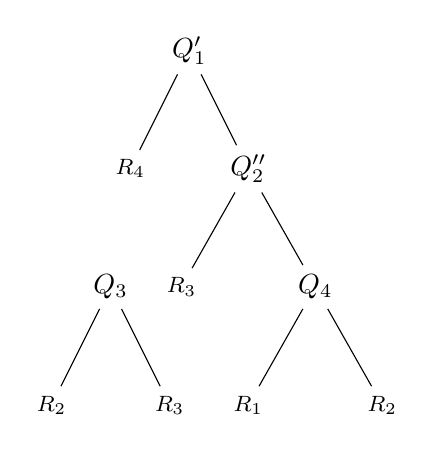
\begin{tikzpicture}[
				level distance=1.5cm,
				level 2/.style={sibling distance=1.7cm}]
				
				\begin{scope}
					\node {$Q_1'$}
					child {node {\footnotesize \texttt{$R_4$}}}
					child {node {$Q_2''$}
						child {node {\footnotesize \texttt{$R_3$}}}
						child {node {$Q_4$}
							child {node {\footnotesize \texttt{$R_1$}}}
							child {node {\footnotesize \texttt{$R_2$}}}
						}
					};
				\end{scope}
				
				\begin{scope}[shift={(-1cm,-3cm)}] % Adjust the shift to position the second graph
					\node {$Q_3$}
					child {node {\footnotesize \texttt{$R_2$}}}
					child {node {\footnotesize \texttt{$R_3$}}};
				\end{scope}
				
				\useasboundingbox (current bounding box.north west) rectangle (current bounding box.south east);
				\node at (current bounding box.south)[below=10pt, text width=9cm, text centered]
				{Dependency Graph};
			\end{tikzpicture}
		\end{minipage}%
		\begin{minipage}{0.49\textwidth}
			\begin{align*}
				Q_1'(x,y,z,w,v) =&\ Q_2(x,y,z,w), R_4(w,v)&\\
				Q_2''(x,y,z,w) =&\ Q_4(x,y,z), R_3(z,w)&\\
				Q_3(y,z,w) =&R_2(y,z), R_3(z,w)&\\
				Q_4(x,y,z) =& R_1(x,y), R_2(y,z)&\\
			\end{align*}
		\end{minipage}
	\end{figure}
\end{frame}

\begin{frame}
	\frametitle{CaVieR}
	\framesubtitle{Cascading View Tree}
	\begin{figure}
		\begin{minipage}{0.4\textwidth}
			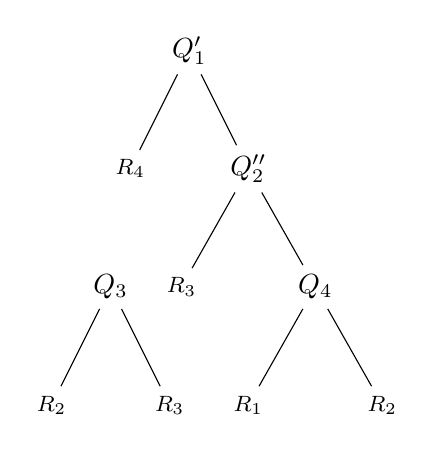
\begin{tikzpicture}[
				level distance=1.5cm,
				level 2/.style={sibling distance=1.7cm}]
				
				\begin{scope}
					\node {$Q_1'$}
					child {node {\footnotesize \texttt{$R_4$}}}
					child {node {$Q_2''$}
						child {node {\footnotesize \texttt{$R_3$}}}
						child {node {$Q_4$}
							child {node {\footnotesize \texttt{$R_1$}}}
							child {node {\footnotesize \texttt{$R_2$}}}
						}
					};
				\end{scope}
				
				\begin{scope}[shift={(-1cm,-3cm)}] % Adjust the shift to position the second graph
					\node {$Q_3$}
					child {node {\footnotesize \texttt{$R_2$}}}
					child {node {\footnotesize \texttt{$R_3$}}};
				\end{scope}
				
				\useasboundingbox (current bounding box.north west) rectangle (current bounding box.south east);
				\node at (current bounding box.south)[below=10pt, text width=9cm, text centered]
				{Dependency Graph};
			\end{tikzpicture}
		\end{minipage}
		\begin{minipage}{0.59\textwidth}
			\textbf{Variable Order} for \\ $Q_2''(x,y,z,w) = Q_4(x,y,z), R_3(z,w)$
			\begin{tikzpicture}[
				level distance=0.7cm,
				sibling distance=0.7cm]
				\node {$z$}
				child {node {$x$}
					child {node {$y$}}
				}
				child {node {$w$}};
			\end{tikzpicture}\\
			\vspace{3cm}
		\end{minipage}
	\end{figure}
\end{frame}

\begin{frame}
	\frametitle{CaVieR}
	\framesubtitle{Cascading View Tree}
	\begin{figure}
		\begin{minipage}{0.4\textwidth}
						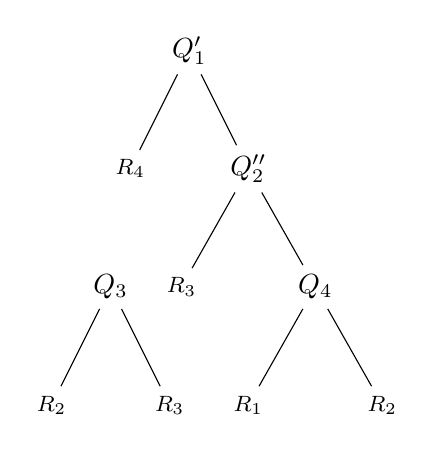
\begin{tikzpicture}[
				level distance=1.5cm,
				level 2/.style={sibling distance=1.7cm}]
				
				\begin{scope}
					\node {$Q_1'$}
					child {node {\footnotesize \texttt{$R_4$}}}
					child {node {$Q_2''$}
						child {node {\footnotesize \texttt{$R_3$}}}
						child {node {$Q_4$}
							child {node {\footnotesize \texttt{$R_1$}}}
							child {node {\footnotesize \texttt{$R_2$}}}
						}
					};
				\end{scope}
				
				\begin{scope}[shift={(-1cm,-3cm)}] % Adjust the shift to position the second graph
					\node {$Q_3$}
					child {node {\footnotesize \texttt{$R_2$}}}
					child {node {\footnotesize \texttt{$R_3$}}};
				\end{scope}
				
				\useasboundingbox (current bounding box.north west) rectangle (current bounding box.south east);
				\node at (current bounding box.south)[below=10pt, text width=9cm, text centered]
				{Dependency Graph};
			\end{tikzpicture}
		\end{minipage}
		\begin{minipage}{0.59\textwidth}
			\textbf{Variable Order} for \\ $Q_2''(x,y,z,w) = Q_4(x,y,z), R_3(z,w)$
			\begin{tikzpicture}[
			level distance=0.7cm,
			sibling distance=0.7cm]
			\node {$z$}
			child {node {$x$}
				child {node {$y$}}
			}
			child {node {$w$}};
		\end{tikzpicture}\\
			\vspace{-0.5cm}
			\textbf{View Tree} for $Q_2''$:\\
			\begin{figure}
				\centering
				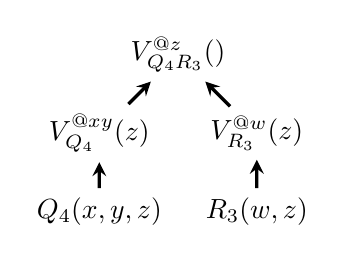
\begin{tikzpicture}[
					level distance=1cm,
					sibling distance=2cm,
	    			edge from parent/.style={draw, <-,very thick,>=stealth}]
					\node {$V_{Q_4R_3}^{@z}()$}
					child {node {$V_{Q_4}^{@xy}(z)$}
						child {node {$Q_4(x,y,z)$}}
					}
					child {node {$V_{R_3}^{@w}(z)$}
						child {node {$R_3(w,z)$}}
					};
				\end{tikzpicture}
			\end{figure}
		\end{minipage}
	\end{figure}
\end{frame}

\begin{frame}
	\frametitle{CaVieR}
	\framesubtitle{Cascading View Tree}
	\begin{figure}
		\begin{minipage}{0.4\textwidth}
						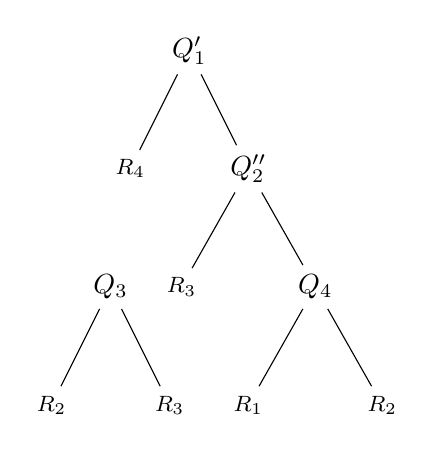
\begin{tikzpicture}[
				level distance=1.5cm,
				level 2/.style={sibling distance=1.7cm}]
				
				\begin{scope}
					\node {$Q_1'$}
					child {node {\footnotesize \texttt{$R_4$}}}
					child {node {$Q_2''$}
						child {node {\footnotesize \texttt{$R_3$}}}
						child {node {$Q_4$}
							child {node {\footnotesize \texttt{$R_1$}}}
							child {node {\footnotesize \texttt{$R_2$}}}
						}
					};
				\end{scope}
				
				\begin{scope}[shift={(-1cm,-3cm)}] % Adjust the shift to position the second graph
					\node {$Q_3$}
					child {node {\footnotesize \texttt{$R_2$}}}
					child {node {\footnotesize \texttt{$R_3$}}};
				\end{scope}
				
				\useasboundingbox (current bounding box.north west) rectangle (current bounding box.south east);
				\node at (current bounding box.south)[below=10pt, text width=9cm, text centered]
				{Dependency Graph};
			\end{tikzpicture}
		\end{minipage}
		\begin{minipage}{0.49\textwidth}
			\vspace{-0.8cm}
			\includegraphics[width=\linewidth]{Figures/CombinedViewTree.pdf}
		\end{minipage}
	\end{figure}
\end{frame}


\begin{frame}
	\frametitle{CaVieR}
	\framesubtitle{Dynamic Evaluation using Cascading View Trees}
	\begin{figure}
		\begin{minipage}{0.5\textwidth}
			\begin{block}{Updates}
				Only relations (not views / queries) receive updates. These updates are only propagated in queries containing them.
			\end{block}
		\end{minipage}
		\begin{minipage}{0.49\textwidth}
			\vspace{-0.8cm}
			\includegraphics[width=\linewidth]{Figures/CombinedViewTree.pdf}
		\end{minipage}
	\end{figure}
\end{frame}

\begin{frame}
	\frametitle{CaVieR}
	\framesubtitle{Dynamic Evaluation using Cascading View Trees}
	\begin{figure}
		\includegraphics[width=0.75\linewidth,trim={0 0 0 11cm},clip]{Figures/CombinedViewTreeD1.pdf}
	\end{figure}
\end{frame}

\begin{frame}
	\frametitle{CaVieR}
	\framesubtitle{Dynamic Evaluation using Cascading View Trees}
	\begin{figure}
		\includegraphics[width=0.75\linewidth,trim={0 0 0 11cm},clip]{Figures/CombinedViewTreeD2.pdf}
	\end{figure}
\end{frame}

\begin{frame}
	\frametitle{CaVieR}
	\framesubtitle{Dynamic Evaluation using Cascading View Trees}
	\begin{figure}
		\includegraphics[width=0.75\linewidth,trim={0 0 0 11cm},clip]{Figures/CombinedViewTreeD3.pdf}
	\end{figure}
\end{frame}

\begin{frame}
	\frametitle{CaVieR}
	\framesubtitle{Dynamic Evaluation using Cascading View Trees}
	\begin{figure}
		\begin{minipage}{0.5\textwidth}
		\begin{block}{Enumeration}
			Enumeration follows the topological order of the queries. Output of a query is turned into a stream of inserts in the view tree of queries that depend on it.
		\end{block}
		\end{minipage}
		\begin{minipage}{0.49\textwidth}
			\vspace{-0.8cm}
			\includegraphics[width=\linewidth]{Figures/CombinedViewTree.pdf}
		\end{minipage}
	\end{figure}
\end{frame}

\begin{frame}
	\frametitle{CaVieR}
	\framesubtitle{Dynamic Evaluation using Cascading View Trees}
	Enumerating $Q_2$
	\begin{figure}
		\begin{tikzpicture}
			\node[anchor=south west,inner sep=0] (image) at (0,0) {\includegraphics[width=0.6\linewidth,trim={0 1.5cm 0 8.5cm},clip]{Figures/CombinedViewTree.pdf}};
			\begin{scope}[x={(image.south east)},y={(image.north west)}]
				\node [anchor=west, blue] at (0.4,0.36) {$y_1$};
			\end{scope}
		\end{tikzpicture}
	\end{figure}
\end{frame}

\begin{frame}
	\frametitle{CaVieR}
	\framesubtitle{Dynamic Evaluation using Cascading View Trees}
	Enumerating $Q_2$
	\begin{figure}
		\begin{tikzpicture}
			\node[anchor=south west,inner sep=0] (image) at (0,0) {\includegraphics[width=0.6\linewidth,trim={0 1.5cm 0 8.5cm},clip]{Figures/CombinedViewTree.pdf}};
			\begin{scope}[x={(image.south east)},y={(image.north west)}]
				\node [anchor=west, blue] at (0.4,0.36) {$y_1$};
				\node [anchor=west, blue] at (0.29,0.21) {$x_1$};
			\end{scope}
		\end{tikzpicture}
	\end{figure}
\end{frame}

\begin{frame}
	\frametitle{CaVieR}
	\framesubtitle{Dynamic Evaluation using Cascading View Trees}
	Enumerating $Q_2$
	\begin{figure}
		\begin{tikzpicture}
			\node[anchor=south west,inner sep=0] (image) at (0,0) {\includegraphics[width=0.6\linewidth,trim={0 1.5cm 0 8.5cm},clip]{Figures/CombinedViewTree.pdf}};
			\begin{scope}[x={(image.south east)},y={(image.north west)}]
				\node [anchor=west, blue] at (0.4,0.36) {$y_1$};
				\node [anchor=west, blue] at (0.29,0.21) {$x_1$};
				\node [anchor=west, blue] at (0.48,0.21) {$z_1$};
			\end{scope}
		\end{tikzpicture}
	\end{figure}
\end{frame}

\begin{frame}
	\frametitle{CaVieR}
	\framesubtitle{Dynamic Evaluation using Cascading View Trees}
	Enumerating $Q_2$
	\begin{figure}
		\begin{tikzpicture}
			\node[anchor=south west,inner sep=0] (image) at (0,0) {\includegraphics[width=0.6\linewidth,trim={0 1.5cm 0 8.5cm},clip]{Figures/CombinedViewTree.pdf}};
			\begin{scope}[x={(image.south east)},y={(image.north west)}]
				\node [anchor=west, blue] at (0.4,0.36) {$y_1$};
				\node [anchor=west, blue] at (0.29,0.21) {$x_1$};
				\node [anchor=west, blue] at (0.48,0.21) {$z_1$};
				\node [anchor=west, red] at (-0.02,0.535) {$(x_1, y_1, z_1) +$};
			\end{scope}
		\end{tikzpicture}
	\end{figure}
\end{frame}

\begin{frame}
	\frametitle{CaVieR}
	\framesubtitle{Dynamic Evaluation using Cascading View Trees}
	Enumerating $Q_2$
	\begin{figure}
		\begin{tikzpicture}
			\node[anchor=south west,inner sep=0] (image) at (0,0) {\includegraphics[width=0.6\linewidth,trim={0 1.5cm 0 8.5cm},clip]{Figures/CombinedViewTree.pdf}};
			\begin{scope}[x={(image.south east)},y={(image.north west)}]
				\node [anchor=west, blue] at (0.4,0.36) {$y_1$};
				\node [anchor=west, blue] at (0.29,0.21) {$x_1$};
				\node [anchor=west, blue] at (0.48,0.21) {$z_1$};
				\node [anchor=west, red] at (-0.02,0.535) {$(x_1, y_1, z_1) +$};
				\node [anchor=west, red] at (-0.2,0.7) {$(z_1 \rightarrow (x_1, y_1)) +$};
			\end{scope}
		\end{tikzpicture}
	\end{figure}
\end{frame}

\subsection{Experiments}
\begin{frame}
	\frametitle{Implementation \& Experiments}
	\framesubtitle{Datasets \& Queries}
	\textbf{Implementation}\\
	Extension of F-IVM, which is based on DBToaster\\
	\vspace{0.1cm}
	\textbf{Datasets}
	\begin{itemize}
		\item TPC-H	  (T...)
		\item JCC-H   (J...)
		\item Retailer  (R...)
	\end{itemize}
	\vspace{1em}
	\textbf{Queries}\\
	\vspace{0.5em}
	\begin{tabular}{c!{\vrule width 2pt}c|c|c}
		$TNQ_4$ & TPC-H & Non Q-Hierarchical  & 4 \rule{0pt}{2.5ex}\\
		\hline \rule{0pt}{2.5ex}
		$JQ_2$ & JCC-H & Q-Hierarchical & 2 \\
	\end{tabular}
	
	\vspace{1em}
	28 Queries total
\end{frame}

\section{Experiments}
\subsection{Hypothesis}
\begin{frame}
	\frametitle{Experiments}
	\framesubtitle{Working Hypothesis}
	\begin{block}{Hypothesis 1 }\label{hyp:initialUpdate}
		CaVieR outperforms F-IVM on Cascading Q-Hierarchical sets of queries with at least one non-q-hierarchical query by having a lower \textbf{update} time.
	\end{block}
	
	\begin{block}{Hypothesis 2}\label{hyp:initialEnumeration}
		CaVieR outperforms F-IVM on Cascading Q-Hierarchical sets of queries with at least one non-q-hierarchical query by having a lower \textbf{enumeration} delay.
	\end{block}

\end{frame}




\begin{frame}
	\frametitle{Experiment 1: Overall Runtime}
	\framesubtitle{Retailer}
	\begin{figure}
		\begin{minipage}{0.25\textwidth}
			\scalebox{0.6}{
				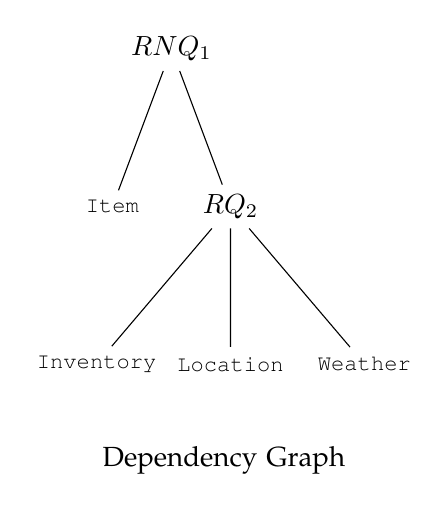
\begin{tikzpicture}[
					level distance=2cm,
					level 2/.style={sibling distance=1.7cm}]
					\node {$RNQ_1$}
					child {node {\footnotesize \texttt{Item}}}
					child {node {$RQ_2$}
						child {node {\footnotesize \texttt{Inventory}}}
						child {node {\footnotesize \texttt{Location}}}
						child {node {\footnotesize \texttt{Weather}}}
					};
					\node at (current bounding box.south)[below=20pt, text width=4cm, text centered]
					{Dependency Graph};
				\end{tikzpicture}
			}
		\end{minipage}
		\begin{minipage}{0.74\textwidth}
			\includegraphics[width=\linewidth]{Figures/hypothesis-retailer} % path to plot 1
		\end{minipage}
		\caption{Incremental maintenance of the results of the query set $\{RNQ_1,\ RQ_2\}$ over the {\em Retailer} dataset under updates of 1000 tuples to all relations. The updates do not follow any specific ordering. }
	\end{figure}
\end{frame}

\begin{frame}
	\frametitle{Experiment 1: Overall Runtime}
	\framesubtitle{TPC-H}
	\begin{figure}		
		\begin{minipage}{0.25\textwidth}
			\scalebox{0.6}{
				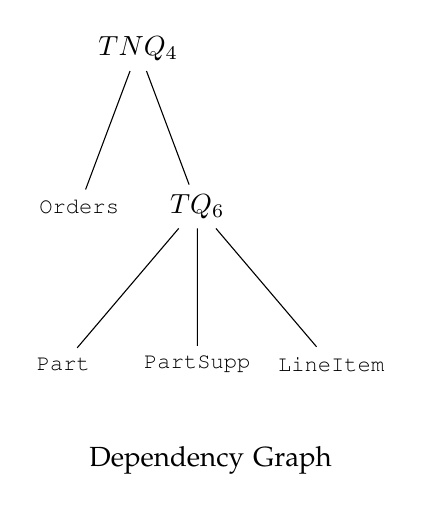
\begin{tikzpicture}[
					level distance=2.0cm,
					level 2/.style={sibling distance=1.7cm}]
					\node {$TNQ_4$}
					child {node {\footnotesize \texttt{Orders}}}
					child {node {$TQ_6$}
						child {node {\footnotesize \texttt{Part}}}
						child {node {\footnotesize \texttt{PartSupp}}}
						child {node {\footnotesize \texttt{LineItem}}}
					};
					\node at (current bounding box.south)[below=20pt, text width=4cm, text centered]
					{Dependency Graph};
				\end{tikzpicture}
			}
		\end{minipage}
		\begin{minipage}{0.74\textwidth}
			\includegraphics[width=\linewidth]{Figures/hypothesis-tpch} % path to plot 1
		\end{minipage}
		\caption{Incremental maintenance of the results of the query set $\{TNQ_4,\ TQ_6\}$ over the {\em TPC-H} dataset.}
	\end{figure}
\end{frame}

\begin{frame}

	\frametitle{Experiment 1: Overall Runtime}
	\framesubtitle{JCC-H}
		\begin{figure}
			\begin{minipage}{0.25\textwidth}
				\scalebox{0.6}{
					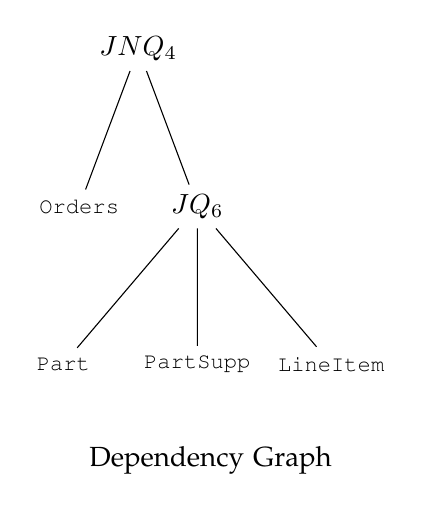
\begin{tikzpicture}[
						level distance=2.0cm,
						level 2/.style={sibling distance=1.7cm}]
						\node {$JNQ_4$}
						child {node {\footnotesize \texttt{Orders}}}
						child {node {$JQ_6$}
							child {node {\footnotesize \texttt{Part}}}
							child {node {\footnotesize \texttt{PartSupp}}}
							child {node {\footnotesize \texttt{LineItem}}}
						};
						\node at (current bounding box.south)[below=20pt, text width=4cm, text centered]
						{Dependency Graph};
					\end{tikzpicture}
				}
			\end{minipage}
			\begin{minipage}{0.74\textwidth}
				\includegraphics[width=\linewidth]{Figures/hypothesis-jcch} % path to plot 1
			\end{minipage}
		\caption{Incremental maintenance of the results of the query set  $\{JNQ_4,\ JQ_6\}$ over the  {\em JCC-H} dataset.
			The results of the queries are enumerated after processing all updates.
		}
		\label{fig:hypothesis}
	\end{figure}
	
\end{frame}



\begin{frame}
	\frametitle{Experiment 2: Many Queries}
	\framesubtitle{TPC-H}
	\begin{figure}
		\begin{minipage}{0.25\textwidth}
			\vspace{1.9cm}
			\scalebox{0.6}{
				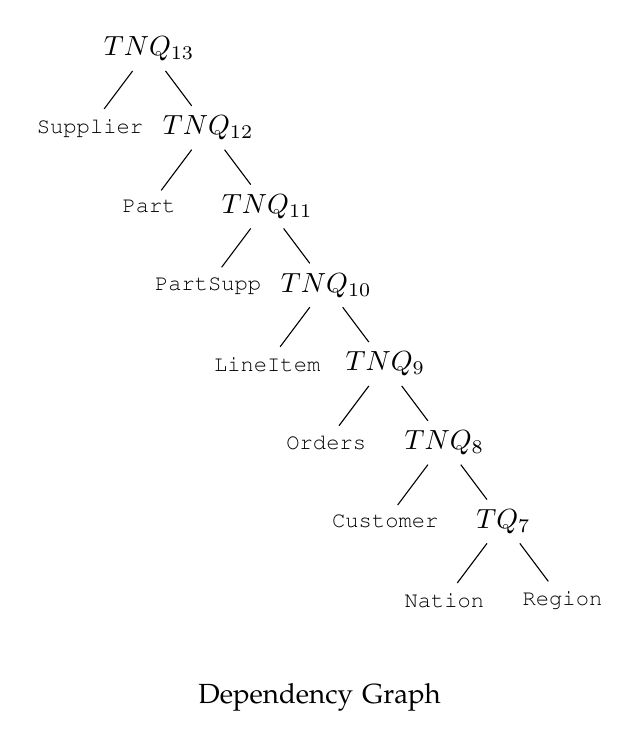
\begin{tikzpicture}[
					level distance=1.0cm,
					level 2/.style={sibling distance=1.5cm}
					]
					\node {$TNQ_{13}$}
					child {node {\footnotesize \texttt{Supplier}}}
					child {node {$TNQ_{12}$}
						child {node {\footnotesize \texttt{Part}}}
						child {node {$TNQ_{11}$}
							child {node {\footnotesize \texttt{PartSupp}}}
							child {node {$TNQ_{10}$}
								child {node {\footnotesize \texttt{LineItem}}}
								child {node {$TNQ_9$}
									child {node {\footnotesize \texttt{Orders}}}
									child {node {$TNQ_8$}
										child {node {\footnotesize \texttt{Customer}}}
										child {node {$TQ_7$}
											child {node {\footnotesize \texttt{Nation}}}
											child {node {\footnotesize \texttt{Region}}}
										}
									}
								}
							}
						}
					};
					\node at (current bounding box.south)[below=20pt, text width=4cm, text centered]
					{Dependency Graph};
				\end{tikzpicture}
			}
		\end{minipage}
		\begin{minipage}{0.74\textwidth}
			\vspace{-2.2cm}
			\begin{figure}
				\includegraphics[width=0.95\linewidth]{Figures/LargeExample1.png}
			\end{figure}
		\end{minipage}
		
	\end{figure}
\end{frame}

\begin{frame}
	\frametitle{Experiment 2: Many Queries}
	\framesubtitle{TPC-H}
	\begin{figure}
		\begin{minipage}{0.2\textwidth}
			\vspace{2cm}
			\scalebox{0.6}{
				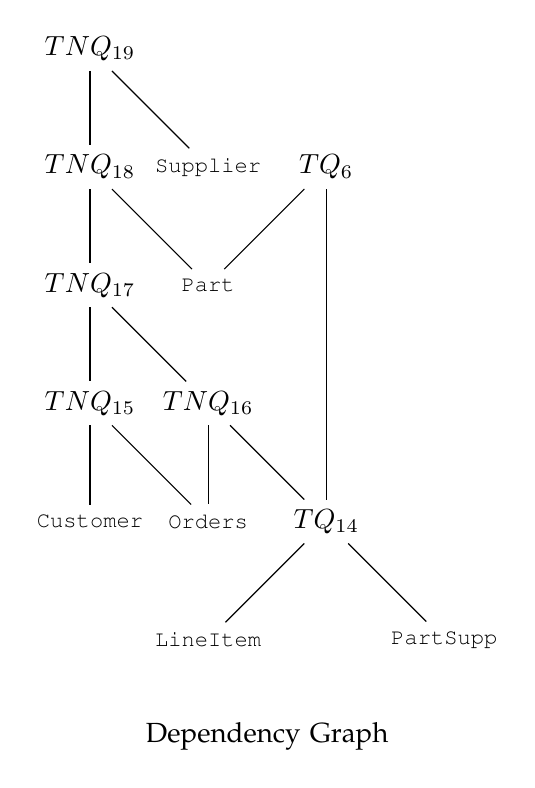
\begin{tikzpicture}[
					level distance=1.0cm,
					node distance=1.5cm
					]
					% Nodes
					\node (TNQ19) {$TNQ_{19}$};
					\node [below of=TNQ19] (TNQ18) {$TNQ_{18}$};
					\node [below of=TNQ18] (TNQ17) {$TNQ_{17}$};
					\node [below of=TNQ18, right of=TNQ18] (Part) {\footnotesize \texttt{Part}};
					\node [right of=TNQ18] (Supplier) {\footnotesize \texttt{Supplier}};
					\node [right of=Supplier] (TQ6) {$TQ_{6}$}; 
					\node [below of=TNQ17] (TNQ15) {$TNQ_{15}$};
					\node [right of=TNQ15] (TNQ16) {$TNQ_{16}$};
					\node [below of=TNQ16, right of=TNQ16] (TQ14) {$TQ_{14}$};
					
					
					% Child nodes
					\node [below of=TQ14,left of=TQ14] (LineItem) {\footnotesize \texttt{LineItem}};
					\node [below of=TNQ15] (Customer) {\footnotesize \texttt{Customer}};
					\node [right of=Customer] (Orders) {\footnotesize \texttt{Orders}};
					\node [below of=TQ14, right of=TQ14] (PartSupp) {\footnotesize \texttt{PartSupp}};
					
					
					
					% Edges
					\draw (TNQ19) -- (TNQ18);
					\draw (TNQ18) -- (TNQ17);
					\draw (TNQ17) -- (TNQ16);
					\draw (TNQ17) -- (TNQ15);
					\draw (TNQ16) -- (TQ14);
					\draw (TQ14) -- (LineItem);
					\draw (TQ14) -- (PartSupp);
					\draw (TNQ15) -- (Orders);
					\draw (TNQ19) -- (Supplier);
					\draw (TNQ18) -- (Part);
					\draw (TQ14) -- (TQ6); 
					\draw (TNQ16) -- (Orders); 
					\draw (TNQ15) -- (Customer); 
					\draw (TQ6) -- (Part); 
					
					% Dependency Graph label
					\node at (current bounding box.south)[below=20pt, text width=4cm, text centered]
					{Dependency Graph};
				\end{tikzpicture}
			}
		\end{minipage}
		\begin{minipage}{0.79\textwidth}
			\vspace{-3cm}
			\begin{figure}
				\includegraphics[width=0.95\linewidth]{Figures/LargeExample2.png}
			\end{figure}
		\end{minipage}
		
	\end{figure}
\end{frame}

\begin{frame}
	\frametitle{Experiments}
	\framesubtitle{Dimensions}
	\begin{itemize}
		\item Data parameters
		\begin{itemize}
			\item Datastream ordering
			\item Cardinalities of the input relations
			\item Value Distribution
		\end{itemize}
		\item Implementation parameters
		\begin{itemize}
			\item Batch size
			\item Payload data structure
		\end{itemize}
		\item Query parameters
		\begin{itemize}
			\item Number of queries
			\item Number of free variables
		\end{itemize}
	\end{itemize}
\end{frame}

\begin{frame}
	\frametitle{Experiment 3: Ordering the Data Stream}
	\framesubtitle{TPC-H}
	\begin{figure}


		\begin{minipage}{0.25\textwidth}
		\scalebox{0.6}{
			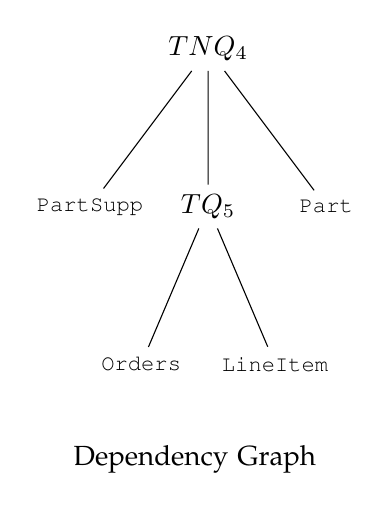
\begin{tikzpicture}[
				level distance=2.0cm,
				level 2/.style={sibling distance=1.7cm}]
				\node {$TNQ_4$}
				child {node {\footnotesize \texttt{PartSupp}}}
				child {node {$TQ_5$}
					child {node {\footnotesize \texttt{Orders}}}
					child {node {\footnotesize \texttt{LineItem}}}
				}
				child {node {\footnotesize \texttt{Part}}};
				\node at (current bounding box.south)[below=20pt, text width=4cm, text centered]
				{Dependency Graph};
			\end{tikzpicture}
		}
		\end{minipage}
		\begin{minipage}{0.74\textwidth}
			\begin{figure}
				\centering
				\includegraphics[width=\linewidth]{Figures/OrderedVSUnordered.png}
			\end{figure}
		\end{minipage}
		\caption{Comparison of the overall update times between ordered and unordered input relations, illustrated using query set $\mathcal{S}_5 = \{TNQ_4,\ TQ_5\}$}
		\label{fig:orderedVSunordered}
	\end{figure}
\end{frame}


\begin{frame}
	\frametitle{Experiment 3: Ordering the Data Stream}
	\framesubtitle{TPC-H}
	\begin{figure}
		\includegraphics[trim={1cm 1.5cm 1cm 1.5cm},clip,width=\linewidth]{Figures/Viz_TPCH_1.pdf}
	\end{figure}
\end{frame}

\begin{frame}
	\frametitle{Hypothesis}
	\framesubtitle{Working Hypothesis}
	\begin{block}{Hypothesis 3}
			CaVieR outperforms F-IVM on Cascading Q-Hierarchical sets of queries with at least one non-q-hierarchical query and \textbf{unordered} input relations by having a lower update time.
	\end{block}
		\begin{block}{Hypothesis 2}
		CaVieR outperforms F-IVM on Cascading Q-Hierarchical sets of queries with at least one non-q-hierarchical query by having a lower enumeration delay.
	\end{block}
	
\end{frame}

\begin{frame}
	\frametitle{Experiment 4: Input Cardinalities}
	\framesubtitle{TPC-H}
	\begin{figure}

		\begin{minipage}{0.25\textwidth}
			\scalebox{0.6}{
				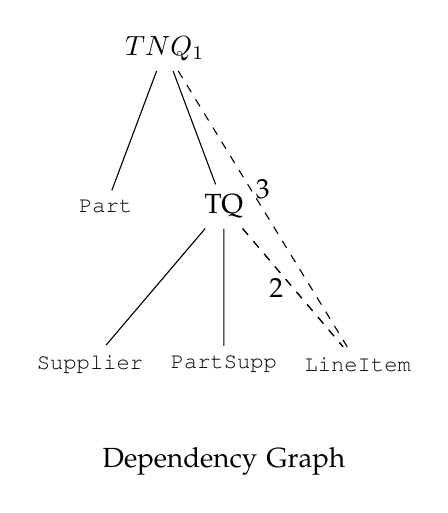
\begin{tikzpicture}[
					level distance=2.0cm,
					level 2/.style={sibling distance=1.7cm}
					]
					\node (TNQ1) {$TNQ_1$}
					child {node {\footnotesize \texttt{Part}}}
					child {node (TQ) {TQ}
						child {node {\footnotesize \texttt{Supplier}}}
						child {node {\footnotesize \texttt{PartSupp}}}
						child[dashed] {node (LineItem) {\footnotesize \texttt{LineItem}}}
					};
					\draw[dashed] (TNQ1) -- (LineItem) node[midway, above] {3};
					\draw[dashed] (TQ) -- (LineItem) node[midway, left] {2};
					\node at (current bounding box.south)[below=20pt, text width=4cm, text centered]
					{Dependency Graph};
				\end{tikzpicture}
			}
		\end{minipage}
		\begin{minipage}{0.74\textwidth}
			\begin{figure}
				\centering
				\includegraphics[width=\linewidth]{Figures/InputCardinalitiesTPCH.png}
			\end{figure}
		\end{minipage}
	\caption{Illustrating the importance of the cardinalities of the individual relations on the update time of both queries in the query sets $\mathcal{S}_3 = \{TNQ_1, TQ_2\}$ \& $\mathcal{S}_4 = \{TNQ_1, TQ_3\}$ on the TPC-H dataset}
\label{fig:inputCardinalitiesTpch}
	\end{figure}
\end{frame}

\begin{frame}
	\frametitle{Experiment 5: Number of Free Variables}
	\framesubtitle{Retailer}
	\begin{figure}
		\begin{minipage}{0.25\textwidth}
			\scalebox{0.6}{
				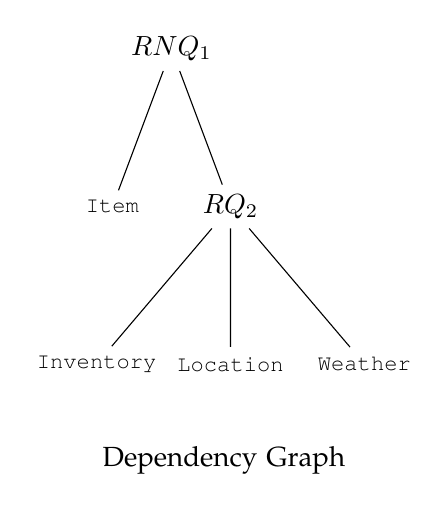
\begin{tikzpicture}[
					level distance=2.0cm,
					level 2/.style={sibling distance=1.7cm}
					]
					\node (RNQ1) {$RNQ_1$}
					child {node {\footnotesize \texttt{Item}}}
					child {node (RQ2) {$RQ_2$}
						child {node {\footnotesize \texttt{Inventory}}}
						child {node {\footnotesize \texttt{Location}}}
						child {node {\footnotesize \texttt{Weather}}}
					};
					\node at (current bounding box.south)[below=20pt, text width=4cm, text centered]
					{Dependency Graph};
				\end{tikzpicture}
			}
		\end{minipage}
		\begin{minipage}{0.74\textwidth}
			\begin{figure}
				\centering
				\includegraphics[width=\linewidth]{Figures/NrFreeVariables.png}
			\end{figure}
		\end{minipage}
	\caption{Influence of the number of free non-join variables on the update time of F-IVM and CaVieR.}
	\label{fig:NrFreeVars}
	\end{figure}
	
\end{frame}

\begin{frame}
	\frametitle{Experiment 6: Influence of skewed Data}
	\framesubtitle{TPC-H \& JCC-H}
		\begin{figure}
		\begin{minipage}{0.25\textwidth}
			\scalebox{0.6}{
				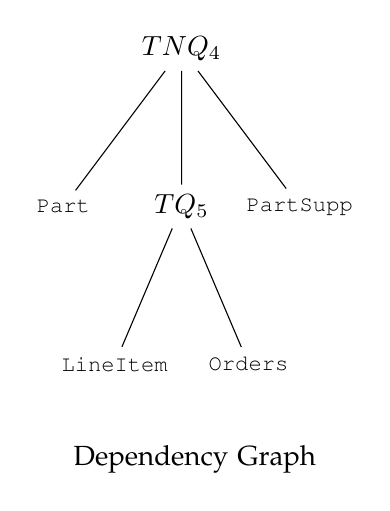
\begin{tikzpicture}[
					level distance=2.0cm,
					level 2/.style={sibling distance=1.7cm}
					]
					\node {$TNQ_4$}
					child {node {\footnotesize \texttt{Part}}}
					child {node {$TQ_5$}
						child {node {\footnotesize \texttt{LineItem}}}
						child {node {\footnotesize \texttt{Orders}}}
					}
					child {node {\footnotesize \texttt{PartSupp}}};
					\node at (current bounding box.south)[below=20pt, text width=4cm, text centered]
					{Dependency Graph};
				\end{tikzpicture}
			}
		\end{minipage}
		\begin{minipage}{0.74\textwidth}
			\begin{figure}
				\centering
				\includegraphics[width=\linewidth]{Figures/TPCH_VS_JCCH.png}
			\end{figure}
		\end{minipage}
		\caption{Comparing TPC-H against JCC-H using CaVieR and F-IVM.}
	\end{figure}
\end{frame}

\begin{frame}
	\frametitle{Experiment 7: Batch Update Sizes}
	\framesubtitle{TPC-H}
	\begin{figure}
		\begin{minipage}{0.25\textwidth}
			\scalebox{0.6}{
				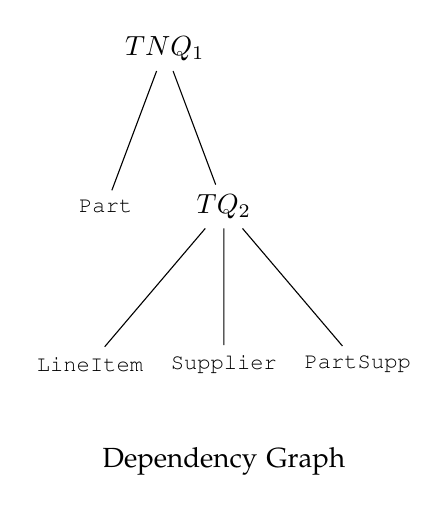
\begin{tikzpicture}[
					level distance=2.0cm,
					level 2/.style={sibling distance=1.7cm}
					]
					\node {$TNQ_1$}
					child {node {\footnotesize \texttt{Part}}}
					child {node {$TQ_2$}
						child {node {\footnotesize \texttt{LineItem}}}
						child {node {\footnotesize \texttt{Supplier}}}
						child {node {\footnotesize \texttt{PartSupp}}}
					};
					\node at (current bounding box.south)[below=20pt, text width=4cm, text centered]
					{Dependency Graph};
				\end{tikzpicture}
			}
		\end{minipage}
		\begin{minipage}{0.74\textwidth}
			\begin{figure}
				\centering
				\includegraphics[width=\linewidth]{Figures/BatchSizes.png}
			\end{figure}
		\end{minipage}
		\caption{Influence of batch sizes on update time. The batch size is given as the base 10 logarithm above each query.}
	\end{figure}
\end{frame}

\begin{frame}
	\frametitle{Experiment 8: Enumeration Delay}
	\framesubtitle{TPC-H}
		\begin{figure}
		\begin{minipage}{0.25\textwidth}
			\scalebox{0.6}{
				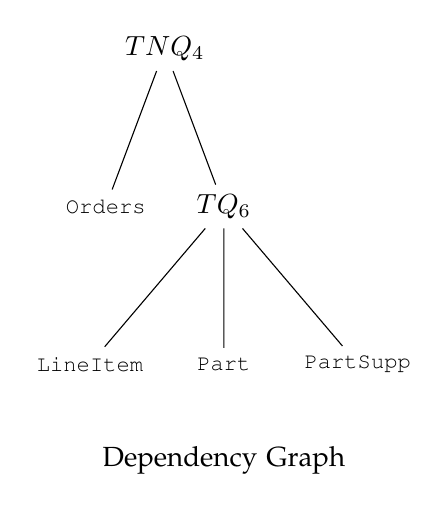
\begin{tikzpicture}[
				level distance=2.0cm,
				level 2/.style={sibling distance=1.7cm}
				]
				\node {$TNQ_4$}
				child {node {\footnotesize \texttt{Orders}}}
				child {node {$TQ_6$}
					child {node {\footnotesize \texttt{LineItem}}}
					child {node {\footnotesize \texttt{Part}}}
					child {node {\footnotesize \texttt{PartSupp}}}
				};
				\node at (current bounding box.south)[below=20pt, text width=4cm, text centered]
				{Dependency Graph};
			\end{tikzpicture}
			}
		\end{minipage}
		\begin{minipage}{0.74\textwidth}
			\begin{figure}
				\centering
				\includegraphics[width=0.7\linewidth]{Figures/EnumerationTimes.png}
			\end{figure}
		\end{minipage}
		\caption{Enumeration times of $TNQ_4$ \& $TQ_6$ compared between F-IVM and CaVieR.}
	\end{figure}
\end{frame}


\begin{frame}
	\frametitle{Experiment 9: Payload Data Structure}
	\framesubtitle{TPC-H}
	\begin{figure}
		\begin{minipage}{0.25\textwidth}
			\scalebox{0.6}{
			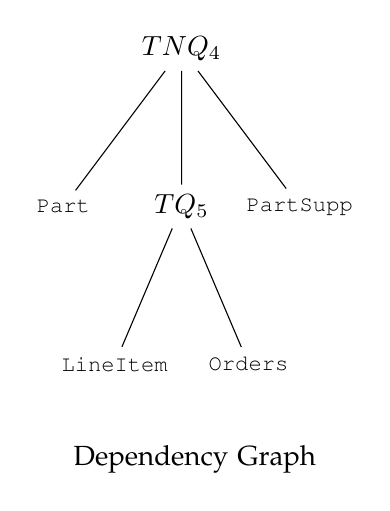
\begin{tikzpicture}[
				level distance=2.0cm,
				level 2/.style={sibling distance=1.7cm}
				]
				\node {$TNQ_4$}
				child {node {\footnotesize \texttt{Part}}}
				child {node {$TQ_5$}
					child {node {\footnotesize \texttt{LineItem}}}
					child {node {\footnotesize \texttt{Orders}}}
				}
				child {node {\footnotesize \texttt{PartSupp}}};
				\node at (current bounding box.south)[below=20pt, text width=4cm, text centered]
				{Dependency Graph};
			\end{tikzpicture}
			}
		\end{minipage}
		\begin{minipage}{0.74\textwidth}
			\begin{figure}
				\centering
				\includegraphics[width=\linewidth]{Figures/MapTypes_tpch.png}
			\end{figure}
		\end{minipage}
		\caption{Comparison of update time \& enumeration delay of the different payload map types on a TPC-H query.}
	\end{figure}
\end{frame}



\begin{frame}
	\frametitle{Experiment 10: Rewriting Q-Hierarchical Queries}
	\framesubtitle{TPC-H}
	\begin{figure}
		\begin{minipage}{0.25\textwidth}
			\scalebox{0.8}{
				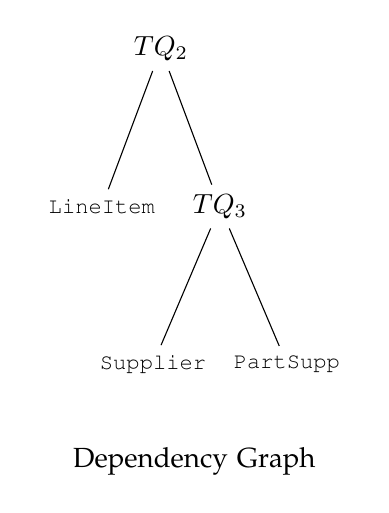
\begin{tikzpicture}[
					level distance=2.0cm,
					level 2/.style={sibling distance=1.7cm}
					]
					\node {$TQ_2$}
					child {node {\footnotesize \texttt{LineItem}}}
					child {node {$TQ_3$}
						child {node {\footnotesize \texttt{Supplier}}}
						child {node {\footnotesize \texttt{PartSupp}}}
					};
					\node at (current bounding box.south)[below=20pt, text width=4cm, text centered]
					{Dependency Graph};
				\end{tikzpicture}
			}
		\end{minipage}
		\begin{minipage}{0.74\textwidth}
			\begin{figure}
				\centering
				\includegraphics[width=0.6\linewidth]{Figures/QHierarchical.png}
			\end{figure}
		\end{minipage}
		\caption{Comparison of update time \& enumeration delay of the different payload map types on a TPC-H query.}
	\end{figure}
\end{frame}


\section{Conclusion}
\subsection{Key Findings}
\begin{frame}
	\frametitle{Key Findings}
	\framesubtitle{Update Time}
	\begin{block}{Data Stream Ordering}
		If the tuples in an update batch share their free variables, the cardinality of the update reduces.
	\end{block}
	\begin{block}{Input Cardinalities}
		If the cardinalities of the relations streamed is unbalanced, reusing the high workload joins is more effective than reusing fast joins.
	\end{block}
	\begin{block}{Free Variables}
		If the cardinalities of the relations streamed is unbalanced, reusing the high workload joins is more effective than reusing fast joins.
	\end{block}
\end{frame}

\begin{frame}
	\frametitle{Key Findings}
	\framesubtitle{Enumeration Delay}
	\begin{block}{Number of Views}
		Using CaVieR, the number of views is smaller or equal to those needed by F-IVM. Thus CaVieR can enumerate the result at least as fast.
	\end{block}
	\begin{block}{Datastructure}
		B+ Trees outperform the other datastructures during enumeration as they support constant time enumeration.
	\end{block}
\end{frame}

\subsection{Future Work}
\begin{frame}
	\frametitle{Future Work }
	\framesubtitle{Comparing Rewritings}
	\begin{align*}
		\colorbox{white}{$Q_1(x,y,z,w)$} =&\  R_1(x,y), R_2(y,z), R_3(z,w)\\
		\colorbox{white}{$Q_2(x,y,z)$} =&\  R_1(x,y), R_2(y,z)\\
		\colorbox{white}{$Q_3(y,z,w)$}=&\ R_2(y,z), R_3(z,w)\\\\
		\color{white}\colorbox{white}{$Q_1'(x,y,z,w)$} =&\color{white}\ Q_2(x,y,z), R_3(z,w)\\
		\color{white}\colorbox{white}{$Q_1''(x,y,z,w)$} =&\color{white}\ R_1(z,w), Q_3(x,y,z)\\
		\color{white}\colorbox{white}{$Q_1'''(x,y,z,w)$} =& \color{white}\ \colorbox{white}{$Q_2(x,y,z)$}, \colorbox{white}{$Q_3(x,y,z)$}
	\end{align*}
\end{frame}
\begin{frame}
	\frametitle{Future Work }
	\framesubtitle{Comparing Rewritings}
	\begin{align*}
		\colorbox{white}{$Q_1(x,y,z,w)$} =&  \colorbox{yellow}{$R_1(x,y), R_2(y,z)$}, R_3(z,w)\\
		\colorbox{orange}{$Q_2(x,y,z)$} =& \colorbox{yellow}{$R_1(x,y), R_2(y,z)$}\\
		\color{gray} \colorbox{white}{$Q_3(y,z,w)$} =&  \color{gray}\ R_2(y,z), R_3(z,w)\\\\
		\colorbox{white}{$Q_1'(x,y,z,w)$} =& \colorbox{orange}{$Q_2(x,y,z)$}, R_3(z,w)\\
		\color{white}\colorbox{white}{$Q_1''(x,y,z,w)$} =&\color{white}\ R_1(z,w), Q_3(x,y,z)\\
		\color{white}\colorbox{white}{$Q_1'''(x,y,z,w)$} =& \color{white}\ \colorbox{white}{$Q_2(x,y,z)$}, \colorbox{white}{$Q_3(x,y,z)$}
	\end{align*}
\end{frame}
\begin{frame}
	\frametitle{Future Work }
	\framesubtitle{Comparing Rewritings}
	\begin{align*}
		\colorbox{white}{$Q_1(x,y,z,w)$} =& R_1(x,y), \colorbox{lightgreen}{$R_2(y,z), R_3(z,w)$}\\
		\color{gray}\colorbox{white}{$Q_2(x,y,z)$} =&  \color{gray}\ R_1(x,y), R_2(y,z)\\
		\colorbox{cyan}{$Q_3(y,z,w)$} =& \colorbox{lightgreen}{$R_2(y,z), R_3(z,w)$}\\\\
		\color{gray}\colorbox{white}{$Q_1'(x,y,z,w)$} =&\color{gray}\ Q_2(x,y,z), R_3(z,w)\\
		\colorbox{white}{$Q_1''(x,y,z,w)$} =&\ R_1(z,w), \colorbox{cyan}{$Q_3(x,y,z)$}\\
		\color{white}\colorbox{white}{$Q_1'''(x,y,z,w)$} =& \color{white}\ \colorbox{white}{$Q_2(x,y,z)$}, \colorbox{white}{$Q_3(x,y,z)$}
	\end{align*}
\end{frame}

\begin{frame}
	\frametitle{Future Work }
	\framesubtitle{Comparing Rewritings}
	\begin{align*}
		\colorbox{white}{$Q_1(x,y,z,w)$} =& \colorbox{yellow}{$R_1(x,y),$}\colorbox{mixed}{$R_2(y,z),$}\colorbox{lightgreen}{$R_3(z,w)$}\\
		\colorbox{orange}{$Q_2(x,y,z)$} =& \colorbox{yellow}{$R_1(x,y), R_2(y,z)$}\\
		\colorbox{cyan}{$Q_3(y,z,w)$} =& \colorbox{lightgreen}{$R_2(y,z), R_3(z,w)$}\\\\
		\color{gray}\colorbox{white}{$Q_1'(x,y,z,w)$} =&\color{gray}\ Q_2(x,y,z), R_3(z,w)\\
		\color{gray}\colorbox{white}{$Q_1''(x,y,z,w)$}  =&\color{gray}\ R_1(z,w), Q_3(x,y,z)\\
		\colorbox{white}{$Q_1'''(x,y,z,w)$} =& \colorbox{orange}{$Q_2(x,y,z)$}, \colorbox{cyan}{$Q_3(x,y,z)$}
	\end{align*}
\end{frame}

\begin{frame}
	\frametitle{Future Work }
	\framesubtitle{Comparing Rewritings}
	\begin{align*}
		Q_1'(x,y,z,w) =& Q_2(x,y,z), R_3(z,w)\\
		Q_1''(x,y,z,w)  =& R_1(z,w), Q_3(x,y,z)\\
		Q_1'''(x,y,z,w) =& Q_2(x,y,z), Q_3(x,y,z)
	\end{align*}
	Which is the fastest ?
	\begin{enumerate}
		\item $\{Q_1', Q_2, Q_3\}$
		\item $\{Q_1'', Q_2, Q_3\}$
		\item $\{Q_1''', Q_2, Q_3\}$
	\end{enumerate}
\end{frame}

\begin{frame}
	\frametitle{Future Work}
	\framesubtitle{Cascading Non-Q-Hierarchical View Trees}
	\begin{block}{Rewrite any Queries if possible}
		\begin{enumerate}
			\item More flexibility
			\item Complex Rewriting selection
			\item No asymptotic gains
		\end{enumerate}
	\end{block}
\end{frame}

\begin{frame}
	\frametitle{Future Work}
	\framesubtitle{Alternative Tree Combination Methods}
	\begin{block}{Reuse shared subtrees without enumeration}
		\begin{enumerate}
			\item Does not reduce asymptotic complexity.
			\item Exactly match the free \& lifted variables
		\end{enumerate}
	\end{block}
	
		\begin{block}{Reuse shared subtrees with enumeration}
		\begin{enumerate}
			\item Requires enumeration of partial viewtree
			\item More flexibility in the free variables
			\item Difficulte performance estimation
		\end{enumerate}
	\end{block}
\end{frame}

\begin{frame}
	\frametitle{Future Work}
	\framesubtitle{Delta Enumerations}
	\begin{block}{Enumerate \& Propagate only the change}
		On each enumeration request only enumerate the new tuples \& add them to previous enumeration requests.
		This accellerates both F-IVM \& CaVieR.
	\end{block}
\end{frame}
%----------------------------------------------------------------------------------------
%	CLOSING SLIDE
%----------------------------------------------------------------------------------------

\begin{frame}[plain] % The optional argument 'plain' hides the headline and footline
	\begin{center}
		{\Huge The End}
		
		\bigskip\bigskip % Vertical whitespace
		
		{\LARGE Questions? Comments?}
	\end{center}
\end{frame}

%----------------------------------------------------------------------------------------

\end{document} 